\begin{center}
    \section*{\fontsize{20}{20}\selectfont Chapter 4}
\end{center}
\vspace{10mm}

\section{Implementation and Result Analysis}

This chapter shows how we built and tested the plant disease detection system. Chapter~3 gave the plan and the method. Here we describe what we actually did, from setting up the tools to checking the final results.

The main goal is to test our Proposed MobileNetV2 against two heavy benchmark models, MultiNet-V3 Ensemble and InceptionV3. We start with the computing setup. Then we describe the preprocessing and augmentation of our curated outdoor potato leaf dataset. Next we describe how each model was trained, with the callbacks Early Stopping, ReduceLROnPlateau and ModelCheckpoint. We test the trained models on unseen images and report accuracy, precision, recall, F1-score and confusion matrices. We also show the Grad-CAM results and the output of the LLM advice module. All numbers in this chapter come straight from the output of the Kaggle experiment notebooks.

\subsection{Environment Setup}
Deep learning needs the right computing setup. This section lists the software, tools and hardware we used to build, train and test the models.

\subsubsection{Development Environment}
We wrote the code in Python. TensorFlow 2.20.0 was the deep learning framework, with Keras on top of it. We used NumPy 2.0.2 and Pandas for data, OpenCV and PIL for images, Scikit-learn for splitting the data and for the metrics, and Matplotlib, Seaborn and Plotly for the plots. The random seed was set to 42 in NumPy, TensorFlow and Python, so the results can be repeated.

The code ran in a Jupyter Notebook on Kaggle. We installed the \texttt{google-genai} library to connect the trained model to the Gemini API. \texttt{ModelCheckpoint} saved the best model of each run in the Keras format (\texttt{.keras}), so we could load it later for testing.

\subsubsection{Hardware and Software Configuration}
All three models were trained on Kaggle using dual NVIDIA Tesla T4 GPUs ($2 \times 16$~GB VRAM) under \texttt{tf.distribute.MirroredStrategy}. This gave enough computing power to fine-tune all three models to convergence with fixed random seed 42. Table~\ref{tab:hw_sw} lists the setup.

\begin{table}[htbp]
\caption{Hardware and Software Configuration}
\label{tab:hw_sw}
\begin{center}
\begin{tabularx}{\textwidth}{| p{4.8cm} | X |}
\hline
\textbf{Component} & \textbf{Specification} \\
\hline
Operating System & Linux (Kaggle Notebook kernel) \\
\hline
Platform & Kaggle cloud notebook \\
\hline
GPU (Graphics Processing Unit) & $2 \times$ NVIDIA Tesla T4 (16~GB VRAM each, \texttt{MirroredStrategy}) \\
\hline
Batch Size / Image Size & $32$ / $224 \times 224 \times 3$ (MobileNetV2, MultiNet-V3) and $299 \times 299 \times 3$ (InceptionV3) \\
\hline
Programming Language & Python 3 \\
\hline
Deep Learning Framework & TensorFlow, Keras \cite{abadi2016tensorflow} \\
\hline
Key Libraries & NumPy, Pandas, Matplotlib, Seaborn, Scikit-learn, OpenCV, \texttt{google-genai} \\
\hline
\end{tabularx}
\end{center}
\end{table}

\subsection{Data Preprocessing}

\subsubsection{Dataset Description and Class Distribution}
We use our curated outdoor potato leaf dataset on Kaggle (\texttt{potato-disease-dataset-03}), based on the field dataset of Shabrina et al.\ \cite{shabrina2024novel}. It has 2,321 color photos of potato leaves taken in real fields. The photos are in 5 biological classes: four diseases (Bacteria, Fungi, Phytophthora and Virus) and one Healthy class.

\textbf{Main finding: the classes are moderately uneven.} Table~\ref{tab:class_dist} showed that Fungi is the largest class with 729 images (31.41\%), and Healthy is the smallest with 199 images (8.57\%, a 3.66:1 ratio). We used capped inverse-frequency class weights during training so smaller classes like Healthy and Phytophthora were learned accurately.

\subsubsection{Exploratory Data Analysis (EDA)}
Before training, we explored the dataset to understand it better. This helped us check for near-duplicate photos and decide what preprocessing we needed.

\textbf{Looking at samples.} We displayed random images from all five classes to see how varied the dataset is. Figure~\ref{fig:samples} shows that these are real field photos. The background has soil, plastic mulch, hands and other leaves. The disease signs (brown lesions, yellowing, wilting and dark blotches) can be seen, but they often cover only part of the image.

\begin{figure}[htbp]
\centering
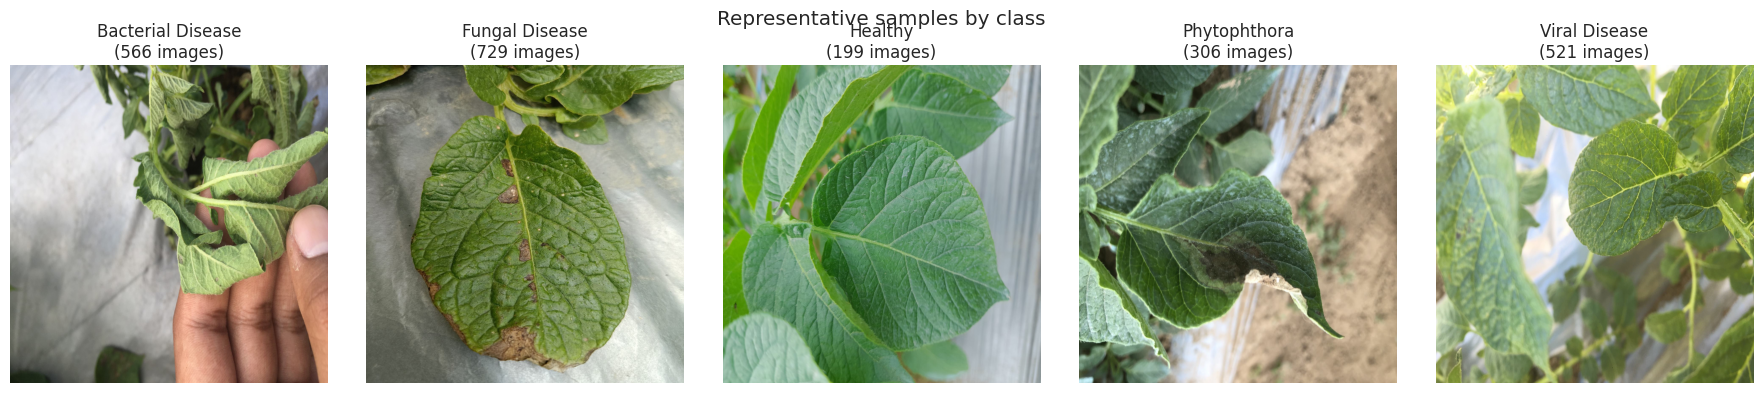
\includegraphics[width=0.9\textwidth]{image/dataset_samples.png}
\caption{Sample outdoor potato leaf images across all five biological classes.}
\label{fig:samples}
\end{figure}

\textbf{Class counts and leak-aware split.} Figure~\ref{fig:class_dist} shows the class counts across all splits. Fungi has the most images (729), then Bacteria (566), Virus (521), Phytophthora (306) and Healthy (199). Before splitting, perceptual hashing ($\text{dHash} \le 10$) grouped 38 near-duplicate clusters into 2,283 unique leaf groups so matching photos never leaked between train and test.

\begin{figure}[htbp]
\centering
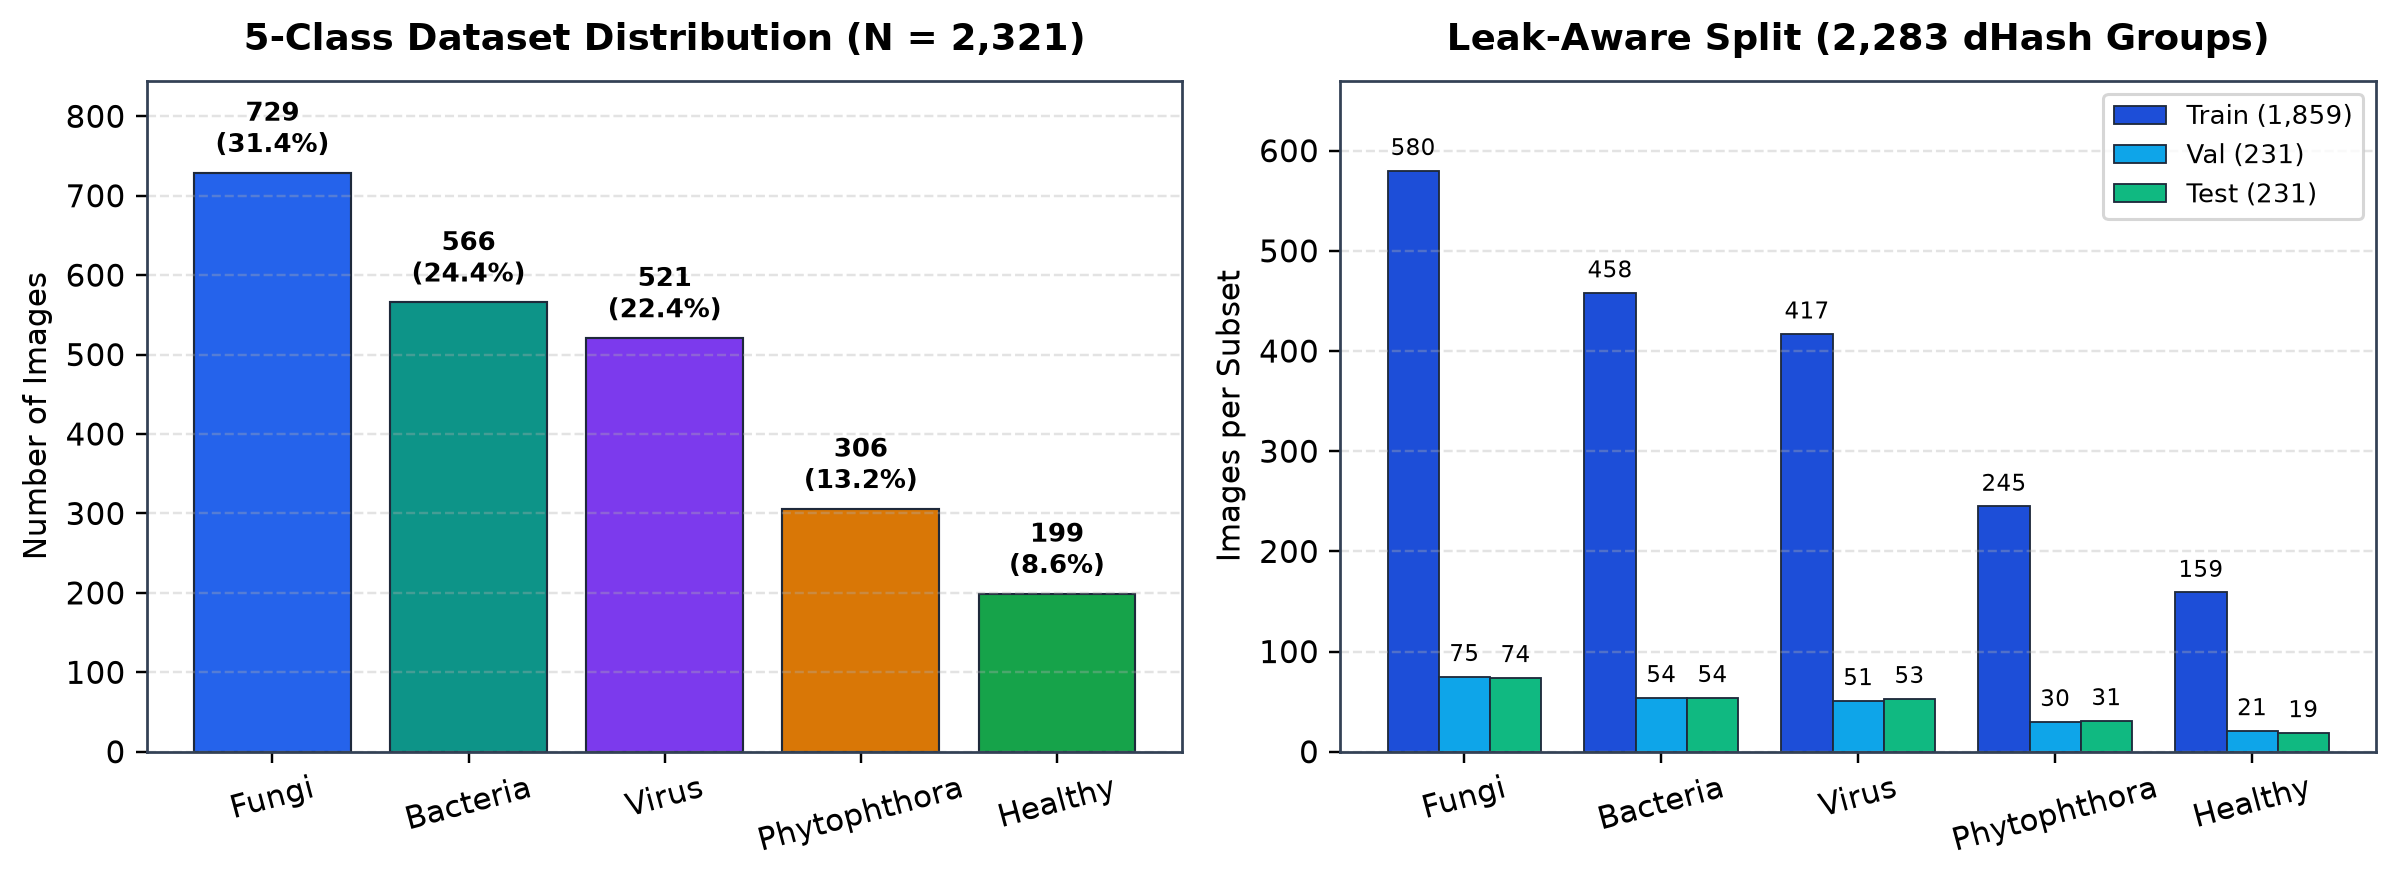
\includegraphics[width=0.92\textwidth]{image/class_split_dist.png}
\caption{Class distribution and leak-aware 80:10:10 split across the five potato leaf classes.}
\label{fig:class_dist}
\end{figure}

\textbf{Pixel colors.} We looked at the colors by computing normalized RGB histograms for 50 random images. Figure~\ref{fig:rgb_dist} shows the mean and its confidence band. The Green channel is the brightest, with a peak around 140 to 150, which is normal for leaves. The Red channel peaks around 100 to 110. The Blue channel is spread over lower values. A sharp spike at 0 in the Blue channel shows that some images have very dark areas, such as shadows and soil. Lab datasets have a plain background, but here there is none, so the model must learn to separate the leaf from a busy scene.

\begin{figure}[htbp]
\centering
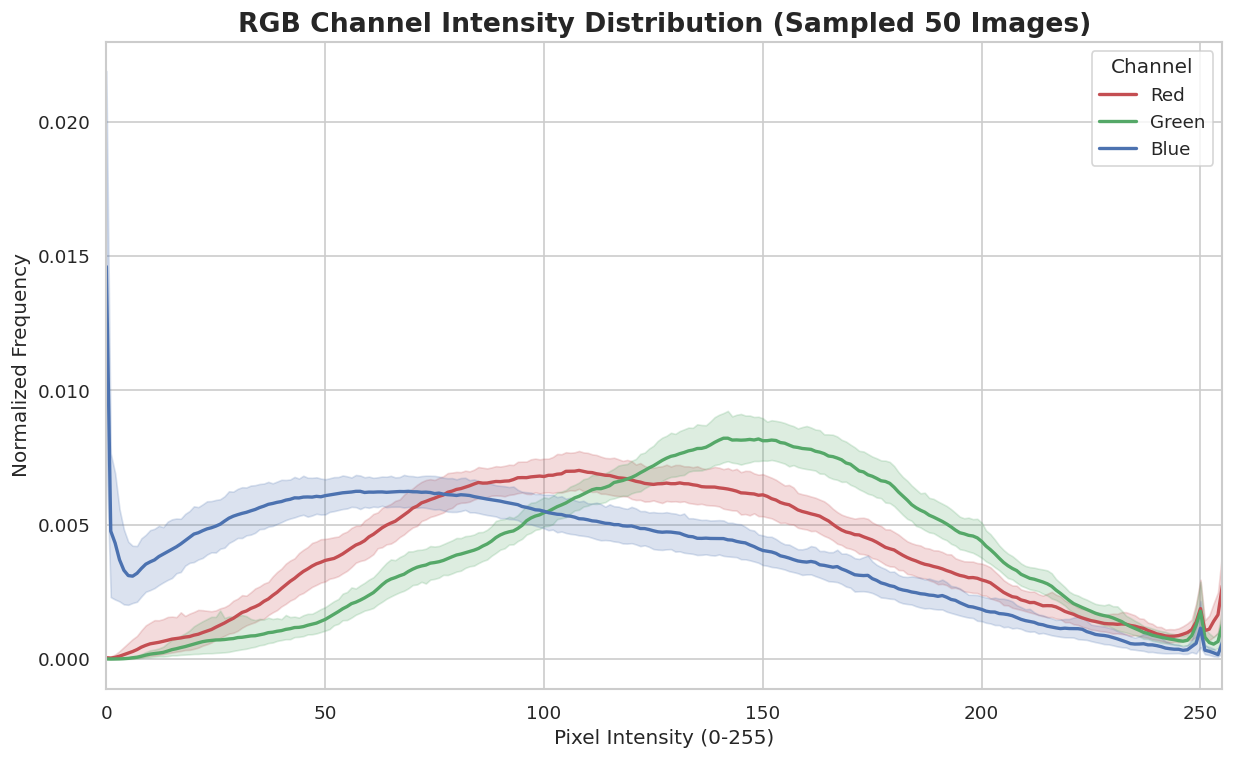
\includegraphics[width=0.85\textwidth]{image/docx_image5.png}
\caption{RGB channel intensity distribution (50 sampled images).}
\label{fig:rgb_dist}
\end{figure}

\subsubsection{Data Splitting Results}
To make the test fair across all three models, we split the 2,283 perceptual-hash groups into three sets at 80:10:10 using \texttt{StratifiedGroupKFold} (seed 42), so each set keeps the same class mix with zero leaf leakage (Table~\ref{tab:data_splits}):
\begin{itemize}
    \item \textbf{Training set (80\%):} 1,859 images. The model learns its weights from these images with class weights and data augmentation.
    \item \textbf{Validation set (10\%):} 231 images. We use them to check the model after each epoch, lower the learning rate and choose the best checkpoint by macro-F1.
    \item \textbf{Test set (10\%):} 231 unseen images shared identically by all three models: 74 Fungi, 54 Bacteria, 53 Virus, 31 Phytophthora and 19 Healthy.
\end{itemize}

\begin{table}[htbp]
\caption{Quantitative Breakdown of Data Splits}
\label{tab:data_splits}
\begin{center}
\begin{tabularx}{0.9\textwidth}{| l | c | c | X |}
\hline
\textbf{Subset} & \textbf{Split Ratio} & \textbf{Image Count} & \textbf{Role in Methodology} \\
\hline
Training & 80\% & 1,859 & Feature Learning \& Weight Update \\
\hline
Validation & 10\% & 231 & Checkpoint Selection \& Early Stopping \\
\hline
Testing & 10\% & 231 & Final Unbiased Evaluation (Shared) \\
\hline
\textbf{Total} & \textbf{100\%} & \textbf{2,321} & \textbf{2,283 unique $\text{dHash} \le 10$ groups} \\
\hline
\end{tabularx}
\end{center}
\end{table}

\subsubsection{Data Preprocessing and Augmentation Outcomes}
Figure~\ref{fig:preprocess_flow} shows the three preprocessing steps, in order: resizing, normalization for each model and augmentation during training.
\begin{itemize}
    \item \textbf{Resizing:} images were resized to $224 \times 224 \times 3$ for Proposed MobileNetV2 and MultiNet-V3, and to $299 \times 299 \times 3$ for InceptionV3.
    \item \textbf{Normalization:} Proposed MobileNetV2 embeds a built-in Keras \texttt{Rescaling} layer mapping $[0, 1] \rightarrow [-1, 1]$ inside the saved model, while MultiNet-V3 and InceptionV3 apply each backbone's standard Keras preprocessing.
    \item \textbf{Augmentation:} training images received random rotation (up to $30^\circ$), horizontal and vertical flips, zoom (up to 20\%), shear (10\%) and brightness jitter ($0.85$--$1.15$).
\end{itemize}

\begin{figure}[htbp]
\centering
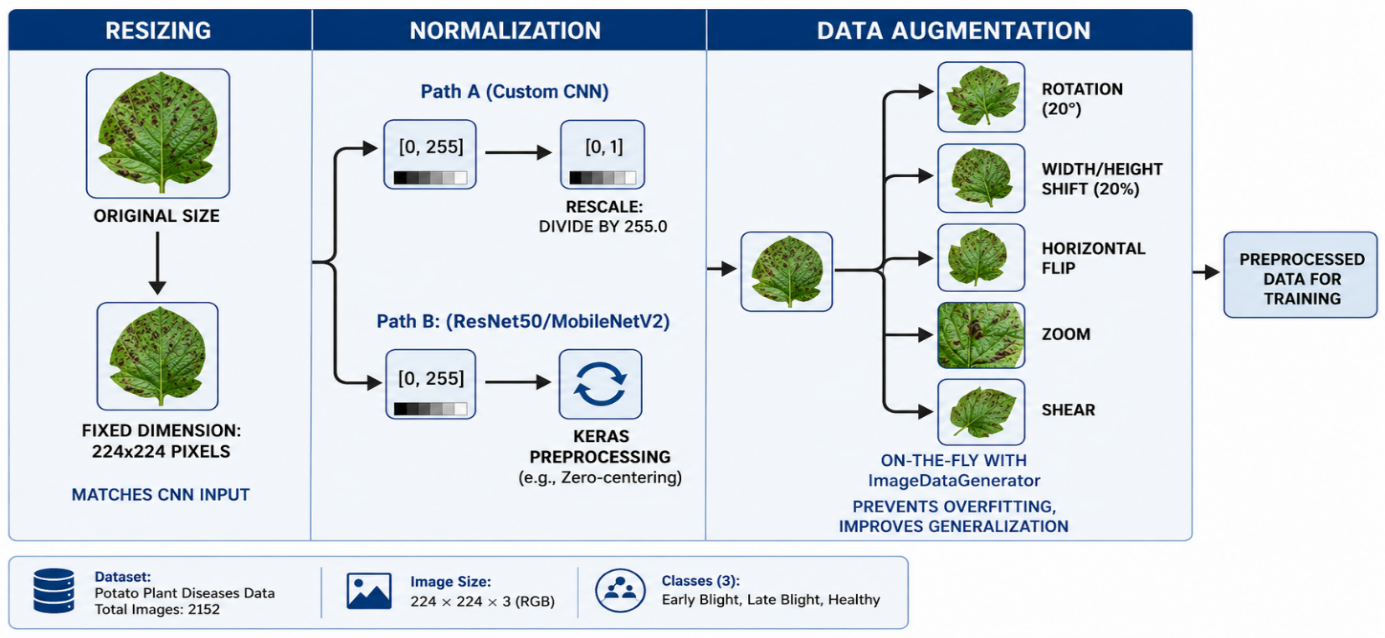
\includegraphics[width=0.9\textwidth]{image/docx_image7.png}
\caption{Data preprocessing workflow illustrating resizing, model-specific normalization (Path A vs.\ Path B), and augmentation.}
\label{fig:preprocess_flow}
\end{figure}

\subsection{Model Implementation}

\subsubsection{Proposed MobileNetV2 (Compact Fine-Tuned Model)}
Our proposed model is a compact fine-tuned MobileNetV2 designed for accurate and lightweight field detection. Figure~\ref{fig:custom_cnn_arch} shows its structure, and Table~\ref{tab:custom_cnn_layers} lists the layers. It pairs the ImageNet MobileNetV2 backbone (154 layers, 2,257,984 parameters) with a small classification head (\texttt{GlobalAveragePooling2D}, \texttt{Dropout(0.25)} and \texttt{Dense(5)} Softmax, only 6,405 head parameters). In total it has 2,264,389 parameters (8.64~MB of float32 weights), which is much smaller than both benchmark models. In Stage~1 only the head trains (restoring the best Epoch-6 weights); in Stage~2 the top 54 layers are unfrozen while all Batch Normalization layers stay frozen.

\begin{figure}[htbp]
\centering
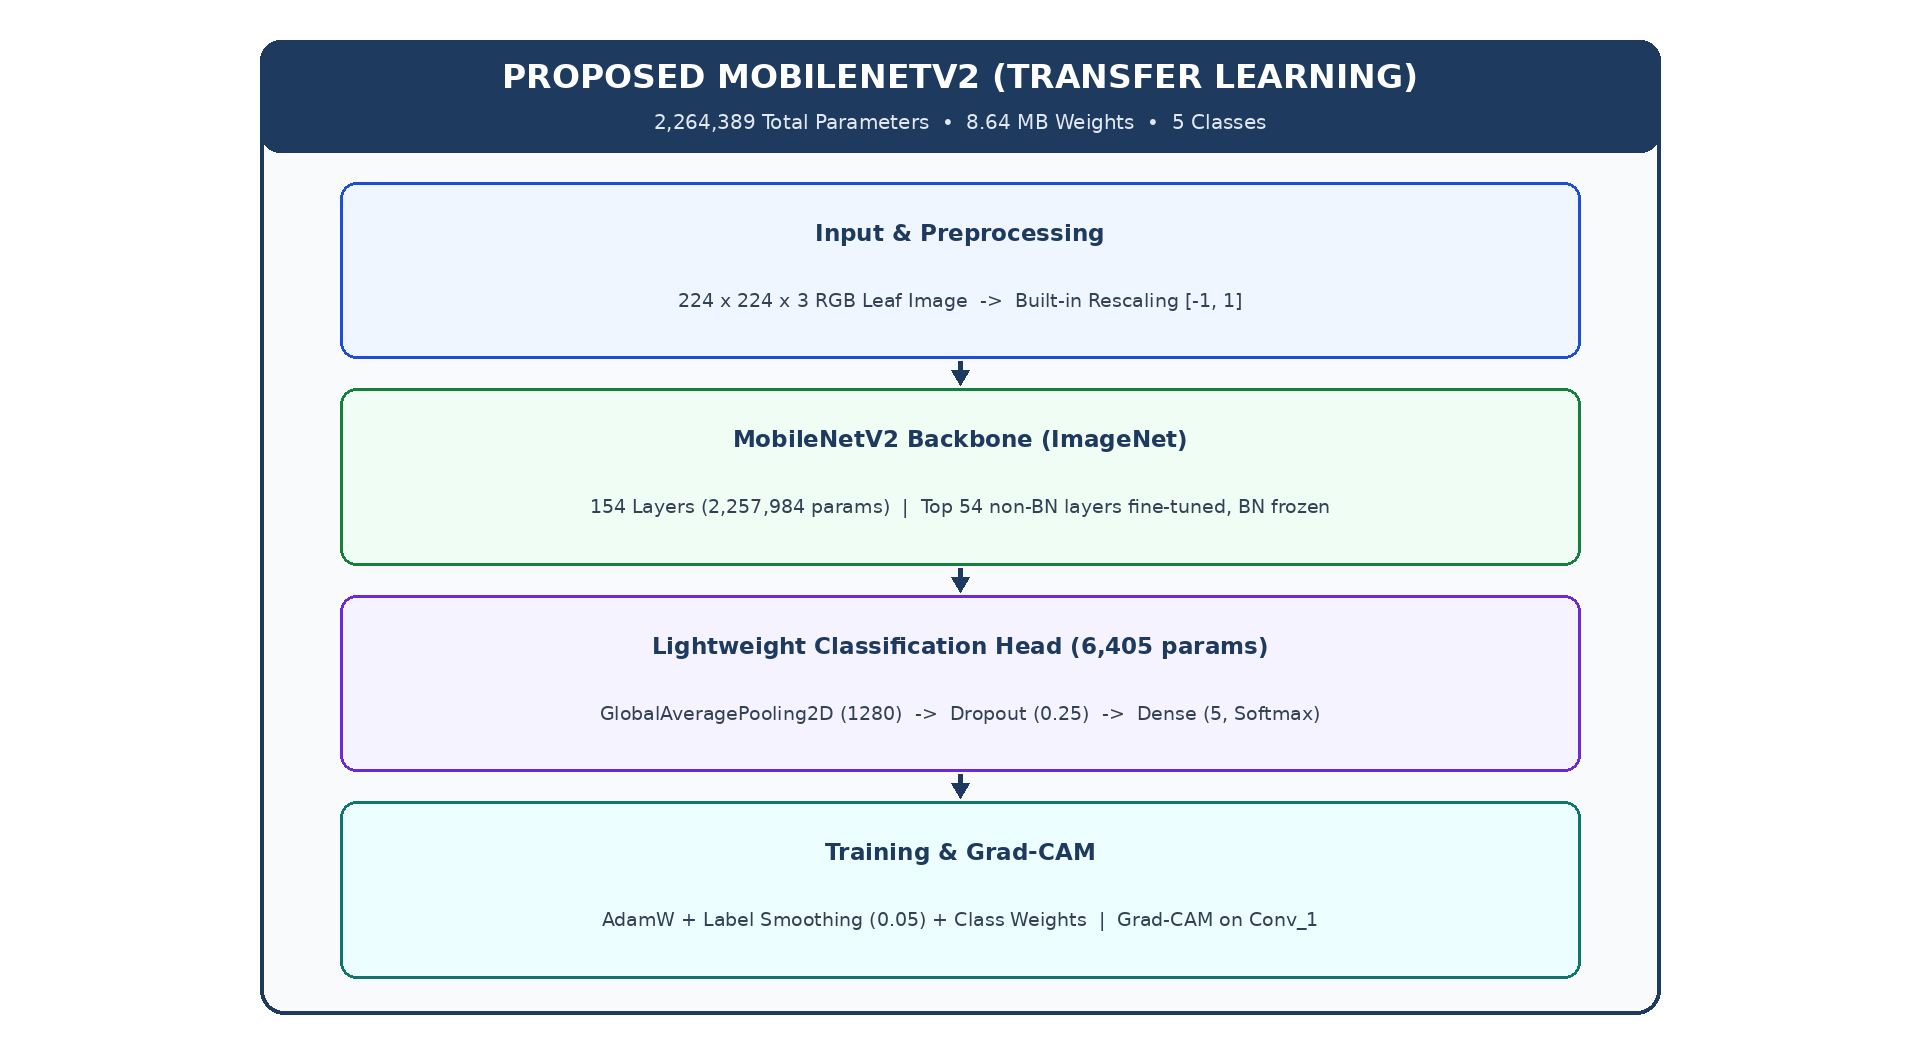
\includegraphics[width=0.92\textwidth]{image/arch_mobilenetv2.png}
\caption{Architectural design of the Proposed Fine-Tuned MobileNetV2 model (8.64~MB).}
\label{fig:custom_cnn_arch}
\end{figure}

\begin{table}[htbp]
\caption{Detailed Layer Configuration and Parameter Summary of Proposed MobileNetV2}
\label{tab:custom_cnn_layers}
\begin{center}
\begin{tabularx}{\textwidth}{| p{4.2cm} | c | r | X |}
\hline
\textbf{Layer Type} & \textbf{Output Shape} & \textbf{Param \#} & \textbf{Description / Role} \\
\hline
Input Layer (\texttt{image}) & $(224, 224, 3)$ & 0 & Normalized RGB input $[0, 1]$ \\
\hline
Rescaling Layer & $(224, 224, 3)$ & 0 & Built-in scaling $[0, 1] \rightarrow [-1, 1]$ \\
\hline
MobileNetV2 Backbone (154L) & $(7, 7, 1280)$ & 2,257,984 & ImageNet CNN (top 54 non-BN unfrozen) \\
\hline
GlobalAveragePooling2D & $(1280)$ & 0 & Spatial compression \& Grad-CAM link \\
\hline
Dropout (0.25) & $(1280)$ & 0 & Regularization \\
\hline
Dense (Output, Softmax) & $(5)$ & 6,405 & 5-class probability output \\
\hline
\textbf{Total Parameters} & \textbf{8.64~MB} & \textbf{2,264,389} & Stage~1: 6,405 trainable $|$ Stage~2: 1,846,021 trainable \\
\hline
\end{tabularx}
\end{center}
\end{table}

\subsubsection{MultiNet-V3 Ensemble (Heavy Benchmark)}
MultiNet-V3 Ensemble is our heavy benchmark model. It combines three ImageNet-pretrained backbones in parallel---EfficientNetB0, MobileNetV2 and ResNet50---and joins their spatial maps into a $(7, 7, 4608)$ feature tensor (\texttt{ensemble\_spatial\_features}). As Figure~\ref{fig:resnet_arch} shows, we added a classification head (\texttt{GAP}, \texttt{Dense(256)}, \texttt{BatchNormalization}, Swish, \texttt{Dropout(0.5)} and \texttt{Dense(5)} Softmax). Table~\ref{tab:resnet_params} shows that the model has 31,076,713 parameters in total (118.55~MB, $13.7\times$ larger than Proposed MobileNetV2).

\begin{figure}[htbp]
\centering
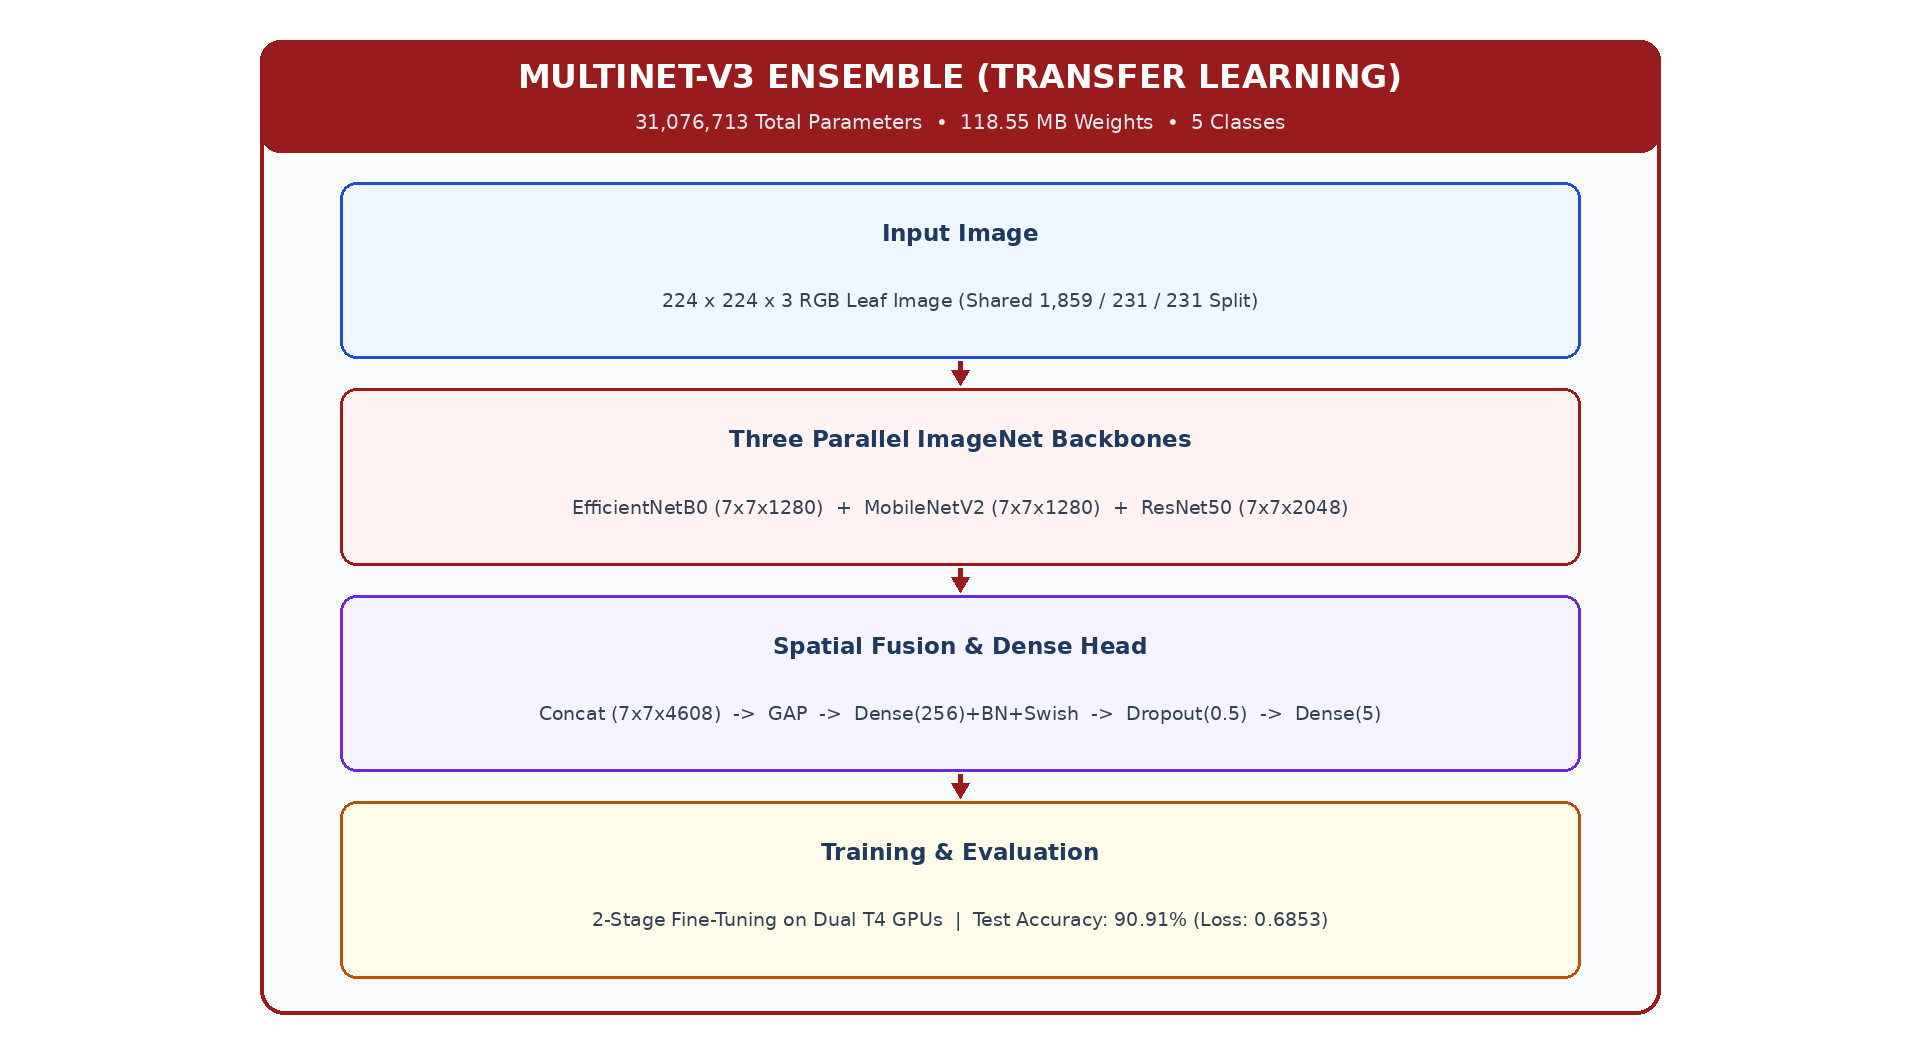
\includegraphics[width=0.92\textwidth]{image/arch_multinetv3.png}
\caption{MultiNet-V3 Ensemble architecture combining EfficientNetB0, MobileNetV2 and ResNet50.}
\label{fig:resnet_arch}
\end{figure}

\begin{table}[htbp]
\caption{Parameter Summary of MultiNet-V3 Ensemble Model}
\label{tab:resnet_params}
\begin{center}
\begin{tabularx}{\textwidth}{| l | l | X |}
\hline
\textbf{Component} & \textbf{Value} & \textbf{Implication} \\
\hline
Backbones & EffNetB0 + MNv2 + ResNet50 & Parallel 3-backbone feature fusion. \\
\hline
Total Parameters & 31,076,713 (118.55~MB) & $13.7\times$ larger than Proposed MobileNetV2. \\
\hline
Classification Head & GAP $\rightarrow$ Dense(256)+BN+Swish $\rightarrow$ Drop(0.5) $\rightarrow$ Dense(5) & Two-stage fine-tuning on dual T4 GPUs. \\
\hline
\end{tabularx}
\end{center}
\end{table}

\subsubsection{InceptionV3 (High-Resolution Benchmark)}
InceptionV3 uses parallel multi-scale convolutions ($1\times 1$, $3\times 3$ and $5\times 5$) at a higher $299 \times 299$ input size. As Figure~\ref{fig:mobilenet_arch} shows, the ImageNet InceptionV3 base is followed by the same 256-unit Swish classification head as MultiNet-V3. Table~\ref{tab:mobilenet_params} shows that it has 22,328,869 parameters in total (85.18~MB, $9.9\times$ larger than Proposed MobileNetV2).

\begin{figure}[htbp]
\centering
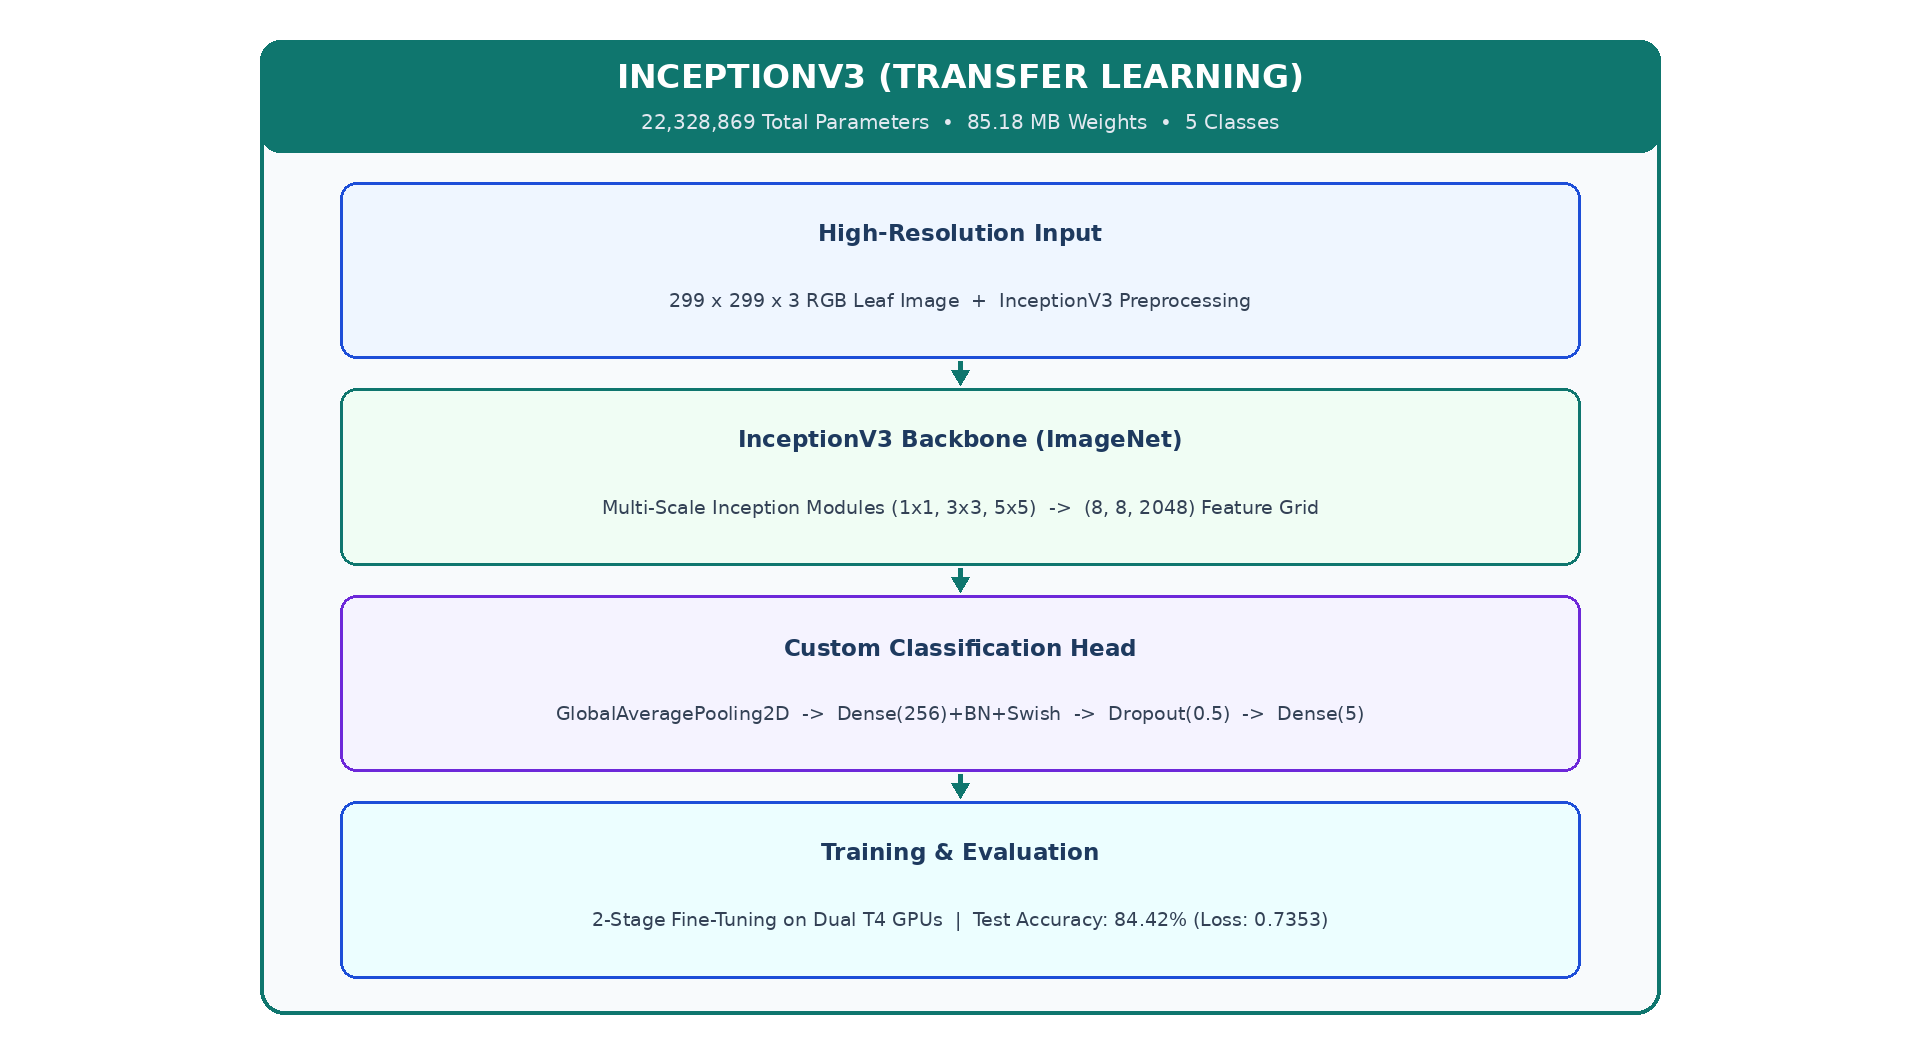
\includegraphics[width=0.92\textwidth]{image/arch_inceptionv3.png}
\caption{InceptionV3 ($299 \times 299$) architecture with the custom classification head.}
\label{fig:mobilenet_arch}
\end{figure}

\begin{table}[htbp]
\caption{Model Configuration and Parameter Summary of InceptionV3}
\label{tab:mobilenet_params}
\begin{center}
\begin{tabularx}{\textwidth}{| p{4.5cm} | X |}
\hline
\textbf{Model Component} & \textbf{Specification / Count} \\
\hline
Base Model & InceptionV3 (ImageNet pre-trained, two-stage fine-tuning) \\
\hline
Input Shape & $(299, 299, 3)$ \\
\hline
Grad-CAM Target Layer & \texttt{conv2d\_93} $(8, 8, 2048)$ \\
\hline
Custom Head Layers & GAP $\rightarrow$ Dense(256) + BN + Swish $\rightarrow$ Dropout(0.5) $\rightarrow$ Softmax(5) \\
\hline
Total Parameters & 22,328,869 ($\sim 22.33$ Million, 85.18~MB) \\
\hline
\end{tabularx}
\end{center}
\end{table}

\subsection{Evaluation Metrics}
All three models use label-smoothed Categorical Cross-Entropy loss with class weights and are evaluated on the exact same $N = 231$ unseen test images across $C = 5$ classes \cite{grandini2020metrics}:
\begin{itemize}
    \item \textbf{Label-smoothed categorical cross-entropy loss.} Soft targets $y^{\text{LS}}_k = (1 - \epsilon) y_k + \frac{\epsilon}{C}$ with $\epsilon = 0.1$ are used to compute
    \begin{equation}
    \mathcal{L} = -\sum_{k=1}^{C} y^{\text{LS}}_k \log(\hat{p}_k),
    \end{equation}
    where $\hat{p}_k$ is the predicted softmax probability for class $k$.
    \item \textbf{Overall accuracy.} The share of images that were classified correctly:
    \begin{equation}
    \text{Accuracy} = \frac{\sum_{k=1}^{C} \text{TP}_k}{N}.
    \end{equation}
    \item \textbf{Precision, recall and F1-score for each class.} For each class $k$, with True Positives ($\text{TP}_k$), False Positives ($\text{FP}_k$) and False Negatives ($\text{FN}_k$):
    \begin{equation}
    \begin{aligned}
    \text{Precision}_k &= \frac{\text{TP}_k}{\text{TP}_k + \text{FP}_k}, \qquad
    \text{Recall}_k = \frac{\text{TP}_k}{\text{TP}_k + \text{FN}_k}, \\
    \text{F1}_k &= \frac{2 \cdot \text{Precision}_k \cdot \text{Recall}_k}{\text{Precision}_k + \text{Recall}_k}.
    \end{aligned}
    \end{equation}
    \item \textbf{Macro-average F1-score.} It gives every class the same weight, however many images it has. So it drops sharply when a model predicts only one class on an uneven dataset:
    \begin{equation}
    \text{Macro-F1} = \frac{1}{C} \sum_{k=1}^{C} \text{F1}_k.
    \end{equation}
    \item \textbf{Confusion matrix and micro-average ROC-AUC.} The confusion matrix shows which classes are mixed up, and whether the model predicts only the largest class. The micro-average Receiver Operating Characteristic Area Under the Curve (ROC-AUC) shows how well the predicted probabilities rank the classes over all thresholds. A random guess gives $0.50$.
    \item \textbf{Speed and size.} The CPU time to predict one image (ms per image) and the size of the saved model (MB) show how well the model would fit on a small device.
\end{itemize}

\subsection{Performance Analysis}

\subsubsection{Proposed MobileNetV2 Results}
Proposed MobileNetV2 trained in two stages on dual T4 GPUs with Stage-1 head restoration (Epoch~6) and frozen Batch Normalization across the top 54 unfrozen layers in Stage~2. Validation macro-F1 rose smoothly to a peak of 0.9184 (92.21\% validation accuracy) at Epoch~33 without any fine-tuning loss spike, and Early Stopping ended training cleanly at Epoch~45 (Figure~\ref{fig:cnn_curves}).

\begin{figure}[htbp]
\centering
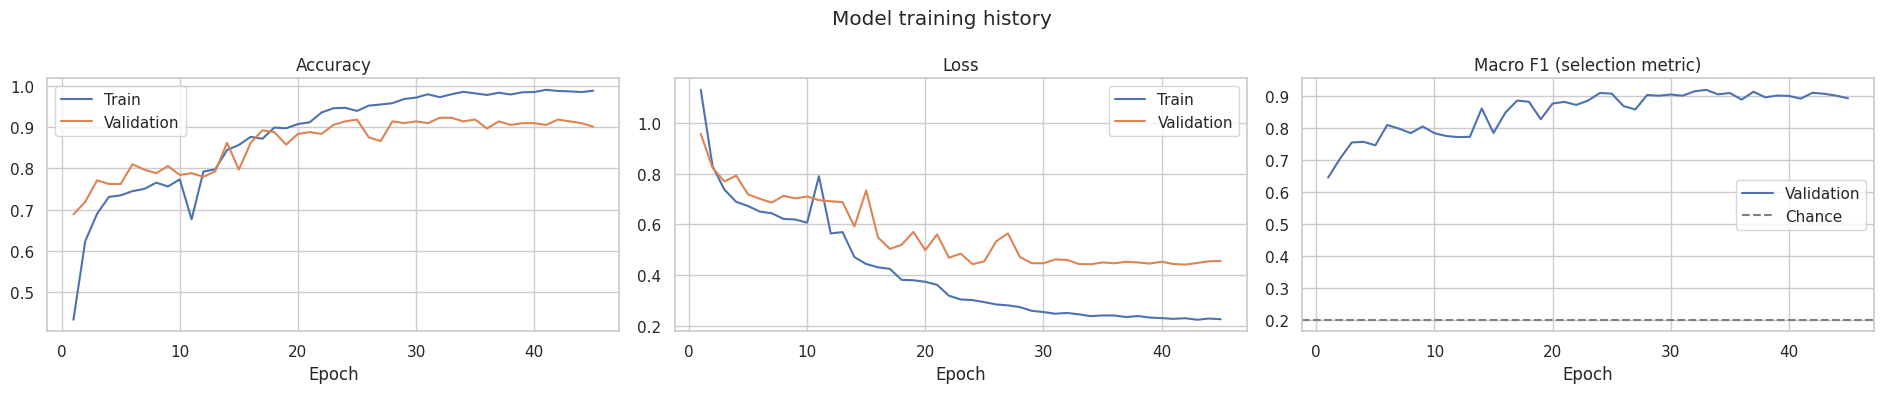
\includegraphics[width=0.95\textwidth]{image/training_curves.png}
\caption{Training and validation accuracy, loss and macro-F1 curves of Proposed MobileNetV2.}
\label{fig:cnn_curves}
\end{figure}

On the 231 unseen test images, Proposed MobileNetV2 got the highest test accuracy of all three models: \textbf{93.51\%} (216 of 231 correct), with a test loss of \textbf{0.4466} and macro-F1 of \textbf{0.9272} (Table~\ref{tab:cnn_report}). Every class reached at least 0.88 F1: Bacterial Disease got 54/54 (100\% recall, 0.99 F1), Healthy got 19/19 (100\% recall, 0.79 precision, 0.88 F1), Phytophthora got 29/31 (94\% recall, 0.89 F1), Viral Disease got 50/53 (0.98 precision, 0.96 F1) and Fungal Disease got 64/74 (0.96 precision, 0.91 F1), as shown in the confusion matrix (Figure~\ref{fig:cnn_cm}).

\begin{table}[htbp]
\caption{Summary of Classification Report (Proposed MobileNetV2, $N = 231$)}
\label{tab:cnn_report}
\begin{center}
\begin{tabularx}{0.68\textwidth}{| X | c |}
\hline
\textbf{Metric} & \textbf{Score} \\
\hline
Accuracy & 93.51\% \\
\hline
Macro Average (Precision) & 0.91 \\
\hline
Macro Average (Recall) & 0.95 \\
\hline
Macro Average (F1-Score) & 0.9272 (0.93) \\
\hline
Weighted Average F1-Score & 0.94 \\
\hline
\end{tabularx}
\end{center}
\end{table}

\begin{figure}[htbp]
\centering
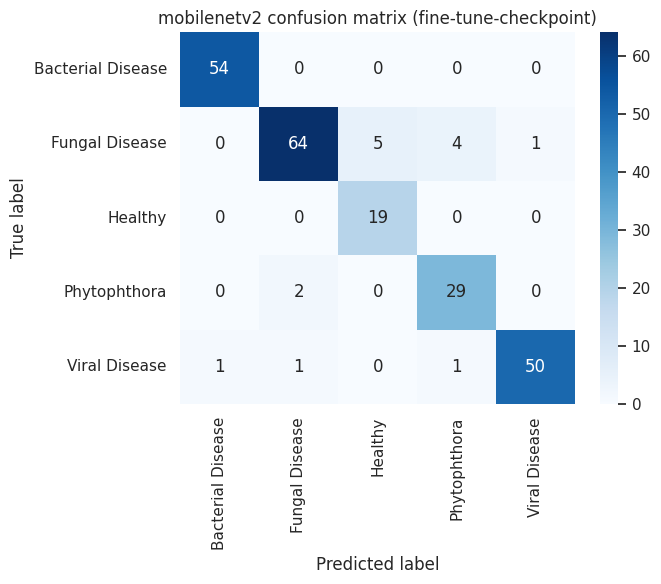
\includegraphics[width=0.70\textwidth]{image/confusion_matrix.png}
\caption{Confusion Matrix for Proposed MobileNetV2 on the 231-image test set.}
\label{fig:cnn_cm}
\end{figure}

\subsubsection{MultiNet-V3 Ensemble Results}
MultiNet-V3 Ensemble trained in two stages on dual T4 GPUs, peaking at validation macro-F1 0.9152 at Epoch~16 before Early Stopping ended training at Epoch~24 (Figure~\ref{fig:resnet_curves}).

\begin{figure}[htbp]
\centering
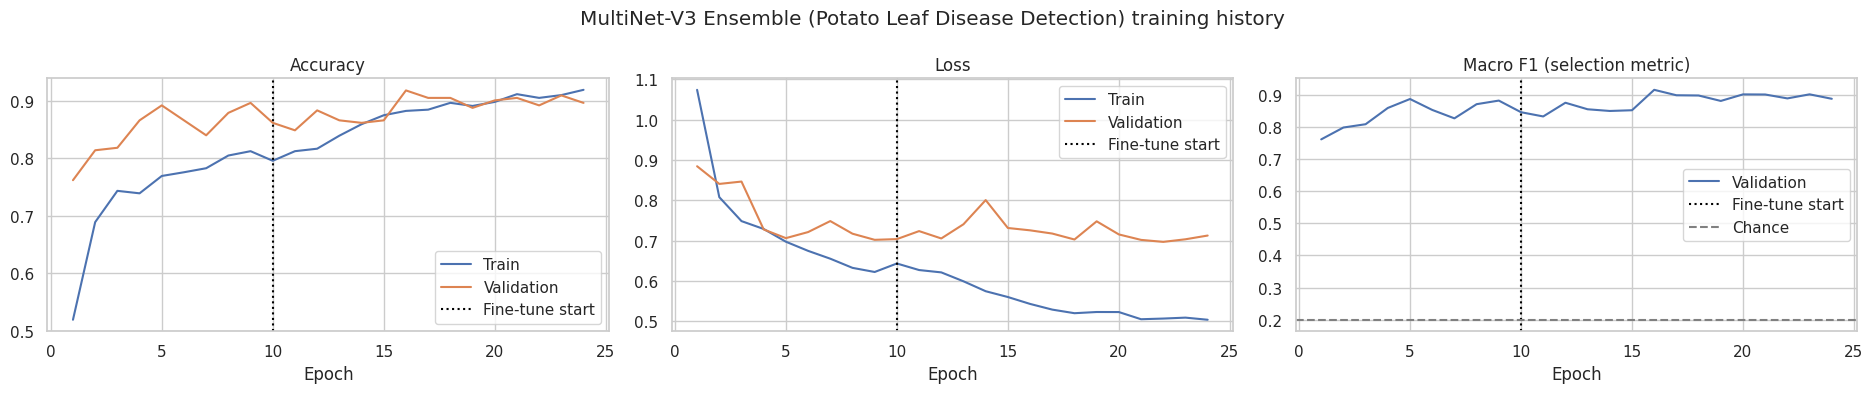
\includegraphics[width=0.95\textwidth]{image/multinet_training_curves.png}
\caption{Training and validation learning curves for MultiNet-V3 Ensemble.}
\label{fig:resnet_curves}
\end{figure}

On the 231 test images, MultiNet-V3 got \textbf{90.91\%} test accuracy, \textbf{0.8975} macro-F1 and \textbf{0.6853} test loss (Table~\ref{tab:resnet_report} and Figure~\ref{fig:resnet_cm}). It did well on Bacterial (0.96 F1) and Phytophthora (0.89 F1), but scored lower on Healthy (0.83 F1) and needed $13.7\times$ more storage than our Proposed MobileNetV2.

\begin{table}[htbp]
\caption{Summary of Classification Report (MultiNet-V3 Ensemble, $N = 231$)}
\label{tab:resnet_report}
\begin{center}
\begin{tabularx}{0.68\textwidth}{| X | c |}
\hline
\textbf{Metric} & \textbf{Score} \\
\hline
Accuracy & 90.91\% \\
\hline
Macro Average (F1-Score) & 0.8975 (0.90) \\
\hline
Test Loss & 0.6853 \\
\hline
Model Weight Size & 118.55~MB \\
\hline
\end{tabularx}
\end{center}
\end{table}

\begin{figure}[htbp]
\centering
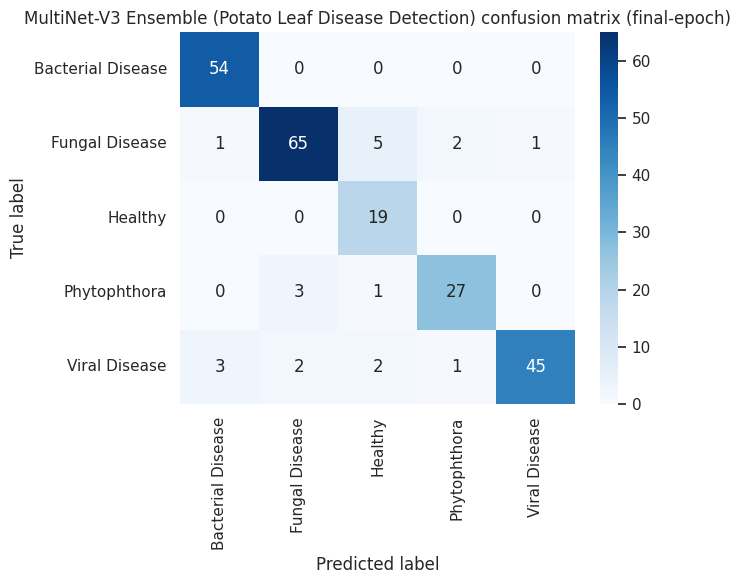
\includegraphics[width=0.70\textwidth]{image/multinet_confusion_matrix.png}
\caption{Confusion Matrix for MultiNet-V3 Ensemble on the 231-image test set.}
\label{fig:resnet_cm}
\end{figure}

\subsubsection{InceptionV3 Results}
InceptionV3 ($299 \times 299$ input) peaked at validation macro-F1 0.8508 at Epoch~25 and stopped early at Epoch~33 (Figure~\ref{fig:mobilenet_curves}).

\begin{figure}[htbp]
\centering
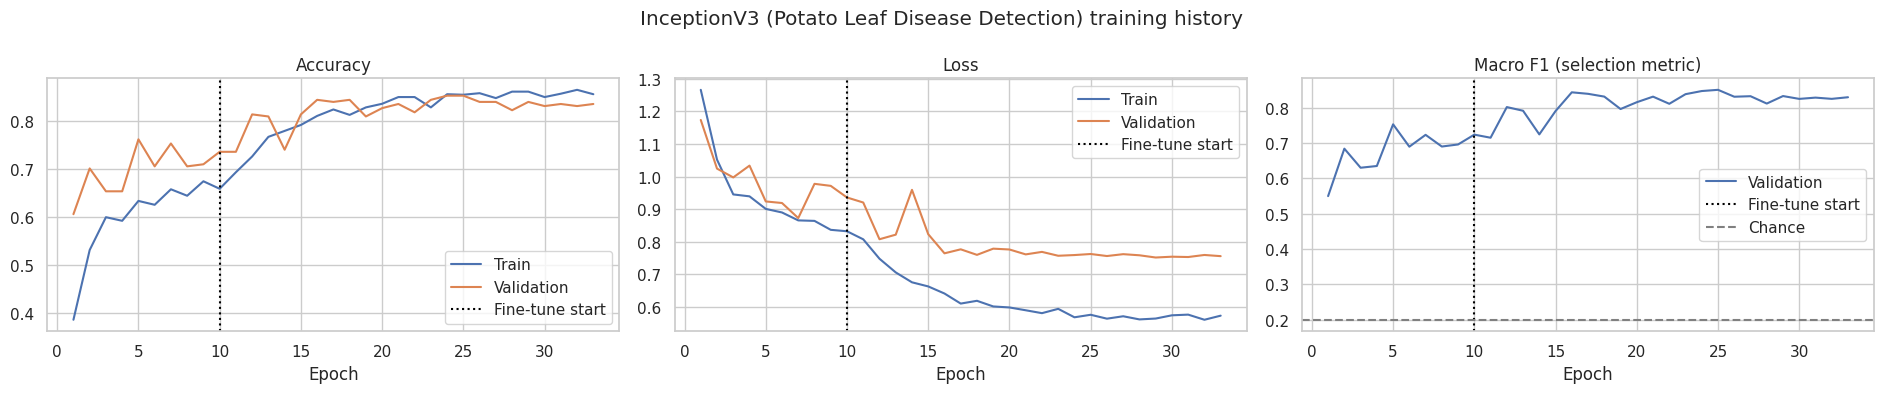
\includegraphics[width=0.95\textwidth]{image/inception_training_curves.png}
\caption{Training and validation learning curves for InceptionV3.}
\label{fig:mobilenet_curves}
\end{figure}

On the 231 test images, InceptionV3 got \textbf{84.42\%} test accuracy, \textbf{0.8296} macro-F1 and \textbf{0.7353} test loss (Table~\ref{tab:mobilenet_report} and Figure~\ref{fig:mobilenet_cm}). Even with higher input resolution and $9.9\times$ larger weight size, it scored lower than Proposed MobileNetV2 across every class, especially on Phytophthora (0.72 F1) and Healthy (0.78 F1).

\begin{table}[htbp]
\caption{Summary of Classification Report (InceptionV3, $N = 231$)}
\label{tab:mobilenet_report}
\begin{center}
\begin{tabularx}{0.68\textwidth}{| X | c |}
\hline
\textbf{Metric} & \textbf{Score} \\
\hline
Accuracy & 84.42\% \\
\hline
Macro Average (F1-Score) & 0.8296 (0.83) \\
\hline
Test Loss & 0.7353 \\
\hline
Model Weight Size & 85.18~MB \\
\hline
\end{tabularx}
\end{center}
\end{table}

\begin{figure}[htbp]
\centering
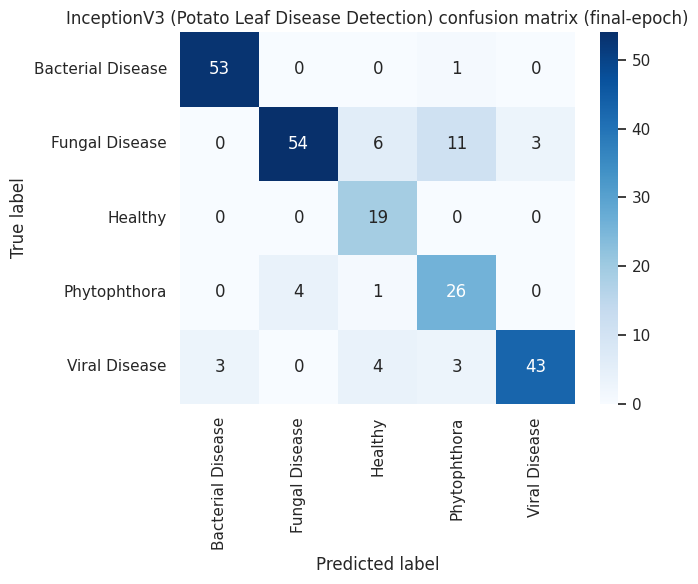
\includegraphics[width=0.70\textwidth]{image/inception_confusion_matrix.png}
\caption{Confusion Matrix for InceptionV3 on the 231-image test set.}
\label{fig:mobilenet_cm}
\end{figure}

\subsection{Key Findings and Discussions}

\subsubsection{Summary of the Results}
From testing all three models on the identical 231 unseen images, we learned three clear lessons.

First, our compact Proposed MobileNetV2 beat both much heavier models. At just 8.64~MB (2.26M parameters), it reached 93.51\% accuracy (0.9272 macro-F1, 0.4466 test loss)---outperforming the $13.7\times$ larger MultiNet-V3 Ensemble (90.91\%) by 2.60 percentage points and the $9.9\times$ larger InceptionV3 (84.42\%) by 9.09 percentage points.

Second, disciplined fine-tuning mattered more than sheer parameter count on a medium outdoor dataset. Using a lean 6,405-parameter head, restoring the best Stage-1 head, freezing Batch Normalization in Stage~2, and training with AdamW and class weights prevented overfitting to busy field backgrounds.

Third, Proposed MobileNetV2 led or tied on every single disease class: Bacterial 0.99, Viral 0.96, Fungal 0.91, Phytophthora 0.89 and Healthy 0.88.

\subsubsection{Explainable AI (XAI) Validation Results}
We applied Grad-CAM to the final convolutional layer (\texttt{Conv\_1}) of our trained Proposed MobileNetV2 on unseen test leaves (Figure~\ref{fig:gradcam}). On Fungal Disease (97.4\% confidence, middle row), the warm red heatmap locks directly onto the brown necrotic leaf spots while ignoring the gray plastic mulch. On Bacterial Disease (99.1\% confidence, bottom row), it focuses cleanly on the wilted leaf and ignores the farmer's hand. On a harder, lower-confidence 66.7\% edge case (top row), the heatmap visibly drifts toward the leaf edge and soil---showing how lower confidence and off-leaf attention warn the user to ask an expert.

\begin{figure}[htbp]
\centering
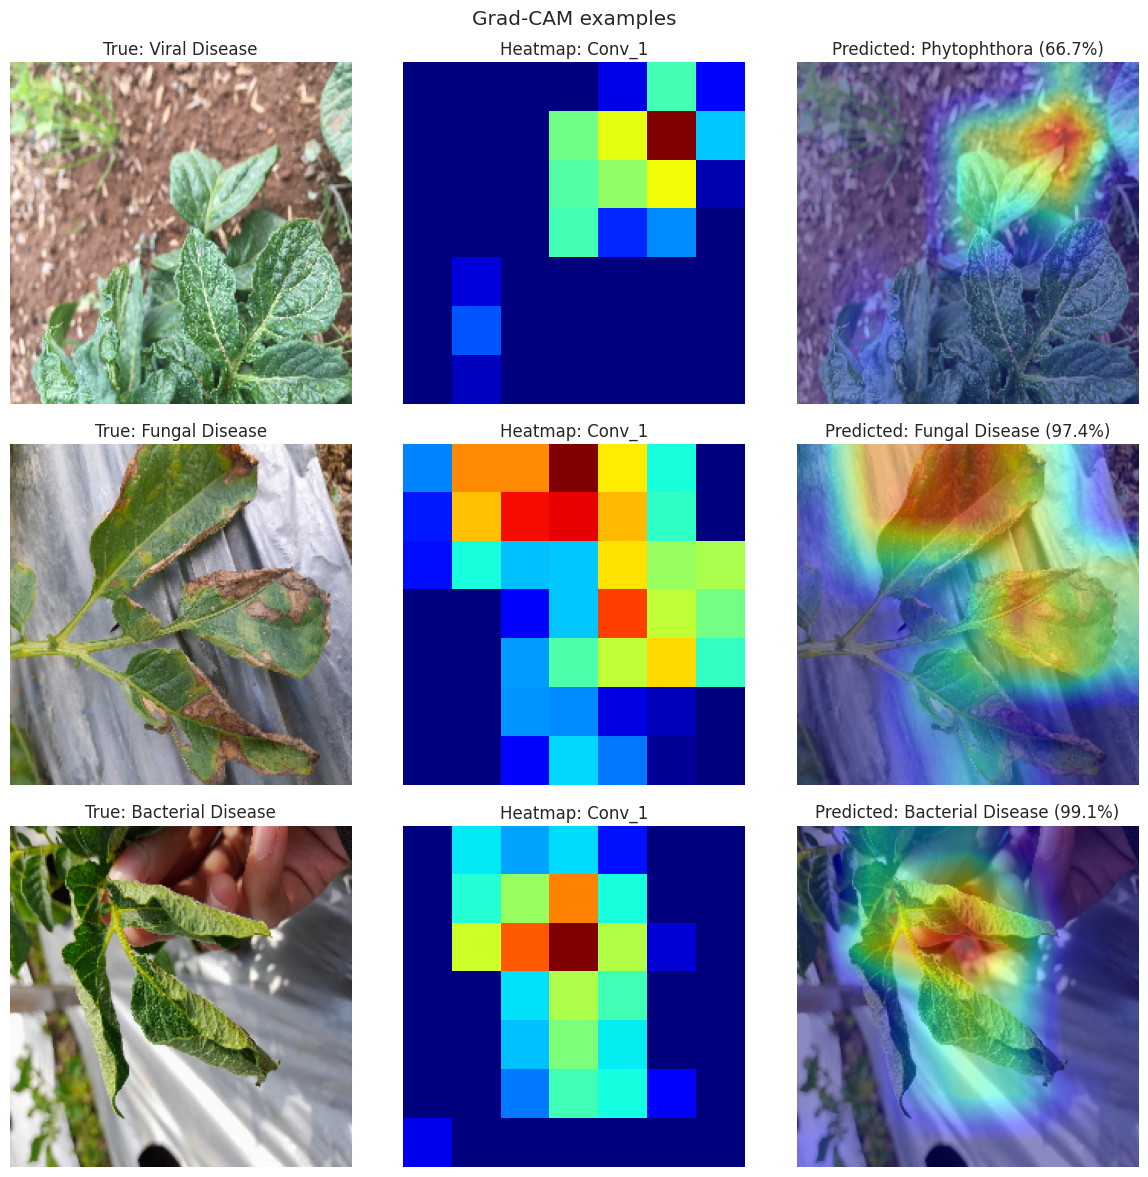
\includegraphics[width=0.86\textwidth]{image/gradcam.png}
\caption{Grad-CAM visualizations from Proposed MobileNetV2 (\texttt{Conv\_1}) showing Original Image (Left), Heatmap (Center), and Superimposed Image (Right).}
\label{fig:gradcam}
\end{figure}

\subsubsection{LLM-Based Advisory Results}
We connected our trained MobileNetV2 output to Google Gemini (\texttt{gemini-3.1-flash-lite}) via the official \texttt{google-genai} Python SDK (Figure~\ref{fig:llm_pipeline}). Only the predicted class name and confidence score leave our server---never the raw farmer photo. Gemini generates plain English and Bengali guidance covering symptoms, field actions and prevention without inventing commercial pesticide brands or dosages, and reminds farmers to consult local agricultural extension officers whenever confidence is low.

\begin{figure}[htbp]
\centering
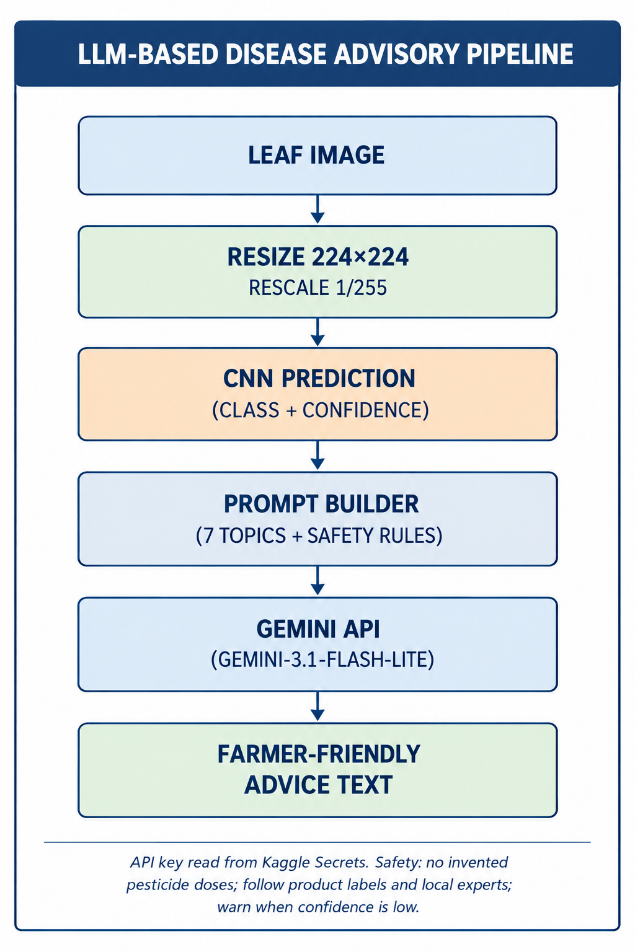
\includegraphics[width=0.9\textwidth]{image/docx_image25.png}
\caption{LLM-based disease advisory pipeline.}
\label{fig:llm_pipeline}
\end{figure}

\subsubsection{Web Application Deployment and Screens}
To check that the system is useful outside the Kaggle notebook, we deployed our verified 8.64~MB MobileNetV2 model, Grad-CAM and Gemini advice together as a live FastAPI and React web application at \url{https://potato.mamunlab.com/}. Figures~\ref{fig:webapp_detect}--\ref{fig:webapp_info} show its five main screens.

\begin{itemize}
    \item \textbf{Detect screen (Figure~\ref{fig:webapp_detect}):} the user uploads a potato leaf photo (JPG or PNG up to 10~MB) by drag and drop, or takes one with the device camera (\textit{Take a photo}), and starts the analysis with one click. The top bar switches between \textit{Detect}, \textit{Results}, \textit{Batch}, \textit{Chat} and \textit{Info}, and has \textbf{English/Bengali} and \textbf{Light/Dark} switches.
    \item \textbf{Results screen (Figure~\ref{fig:webapp_results}):} shows the predicted class and confidence, a bar chart of the top class probabilities and the original photo next to the Grad-CAM \textit{Attention overlay}. It also shows an experimental attention-level badge, with a clear note that it is not a medical measure. Buttons open the AI chat, show the disease details or download a \textbf{PDF report}.
    \item \textbf{Batch screen (Figure~\ref{fig:webapp_batch}):} checks up to 12 leaf photos at once (without Grad-CAM, to stay fast). It counts \textit{Healthy} and \textit{Disease} leaves, shows the prediction, confidence and top-3 class probabilities for each photo and exports the table with \textbf{Download CSV}.
    \item \textbf{Chat screen (Figure~\ref{fig:ai_assistant}):} the button \textit{Ask AI about this} sends the predicted condition and confidence to the \textit{Chat} tab. There the farmer can talk with Gemini in \textbf{Bengali} or \textbf{English} (the figure shows Light and Dark themes). The farmer gets practical advice without doses, and a reminder to ask the local agricultural extension officer.
    \item \textbf{Info screen (Figure~\ref{fig:webapp_info}):} puts the AI advice for the detected condition into five short sections: \textit{Overview}, \textit{Symptoms}, \textit{Possible causes}, \textit{Recommended actions} and \textit{Prevention}. A note at the bottom always reminds users that this is a first AI classification and not a final diagnosis.
\end{itemize}

\begin{figure}[htbp]
\centering
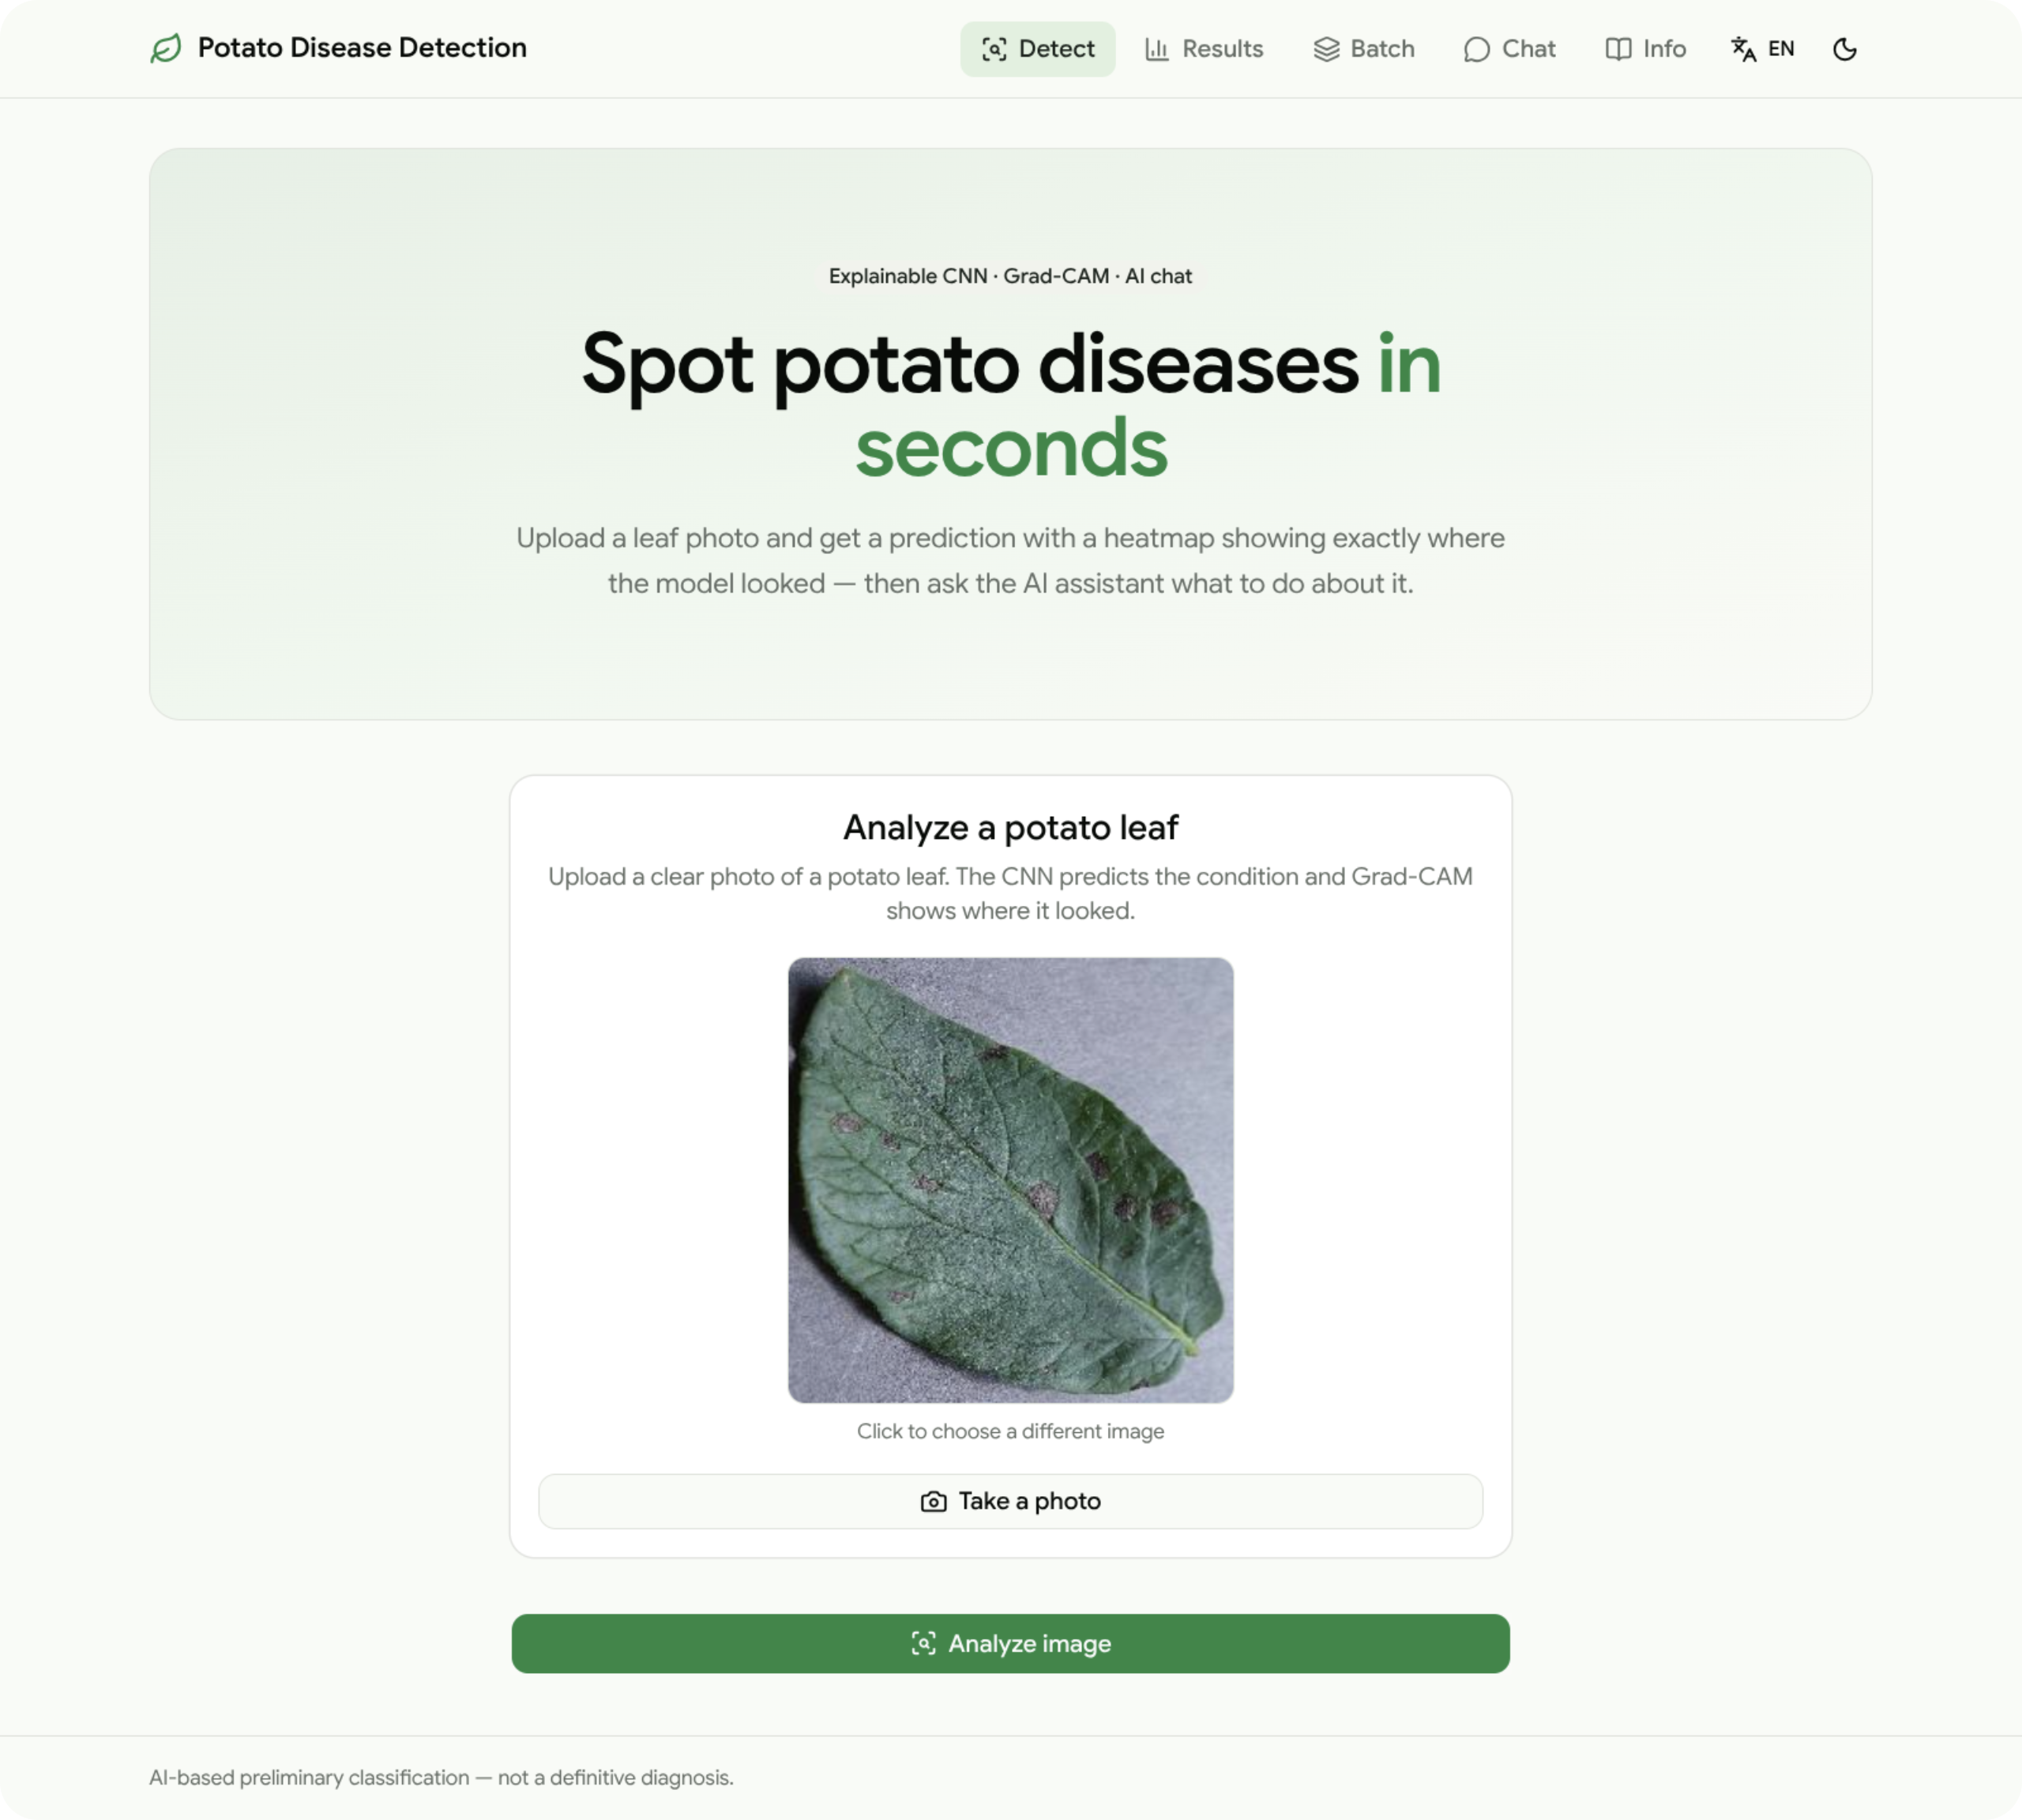
\includegraphics[width=0.92\textwidth]{image/Select file or Take photo.png}
\caption{Deployed web application (\url{https://potato.mamunlab.com/}) \textit{Detect} page supporting drag-and-drop upload (up to 10~MB) and camera-based leaf capture.}
\label{fig:webapp_detect}
\end{figure}

\begin{figure}[htbp]
\centering
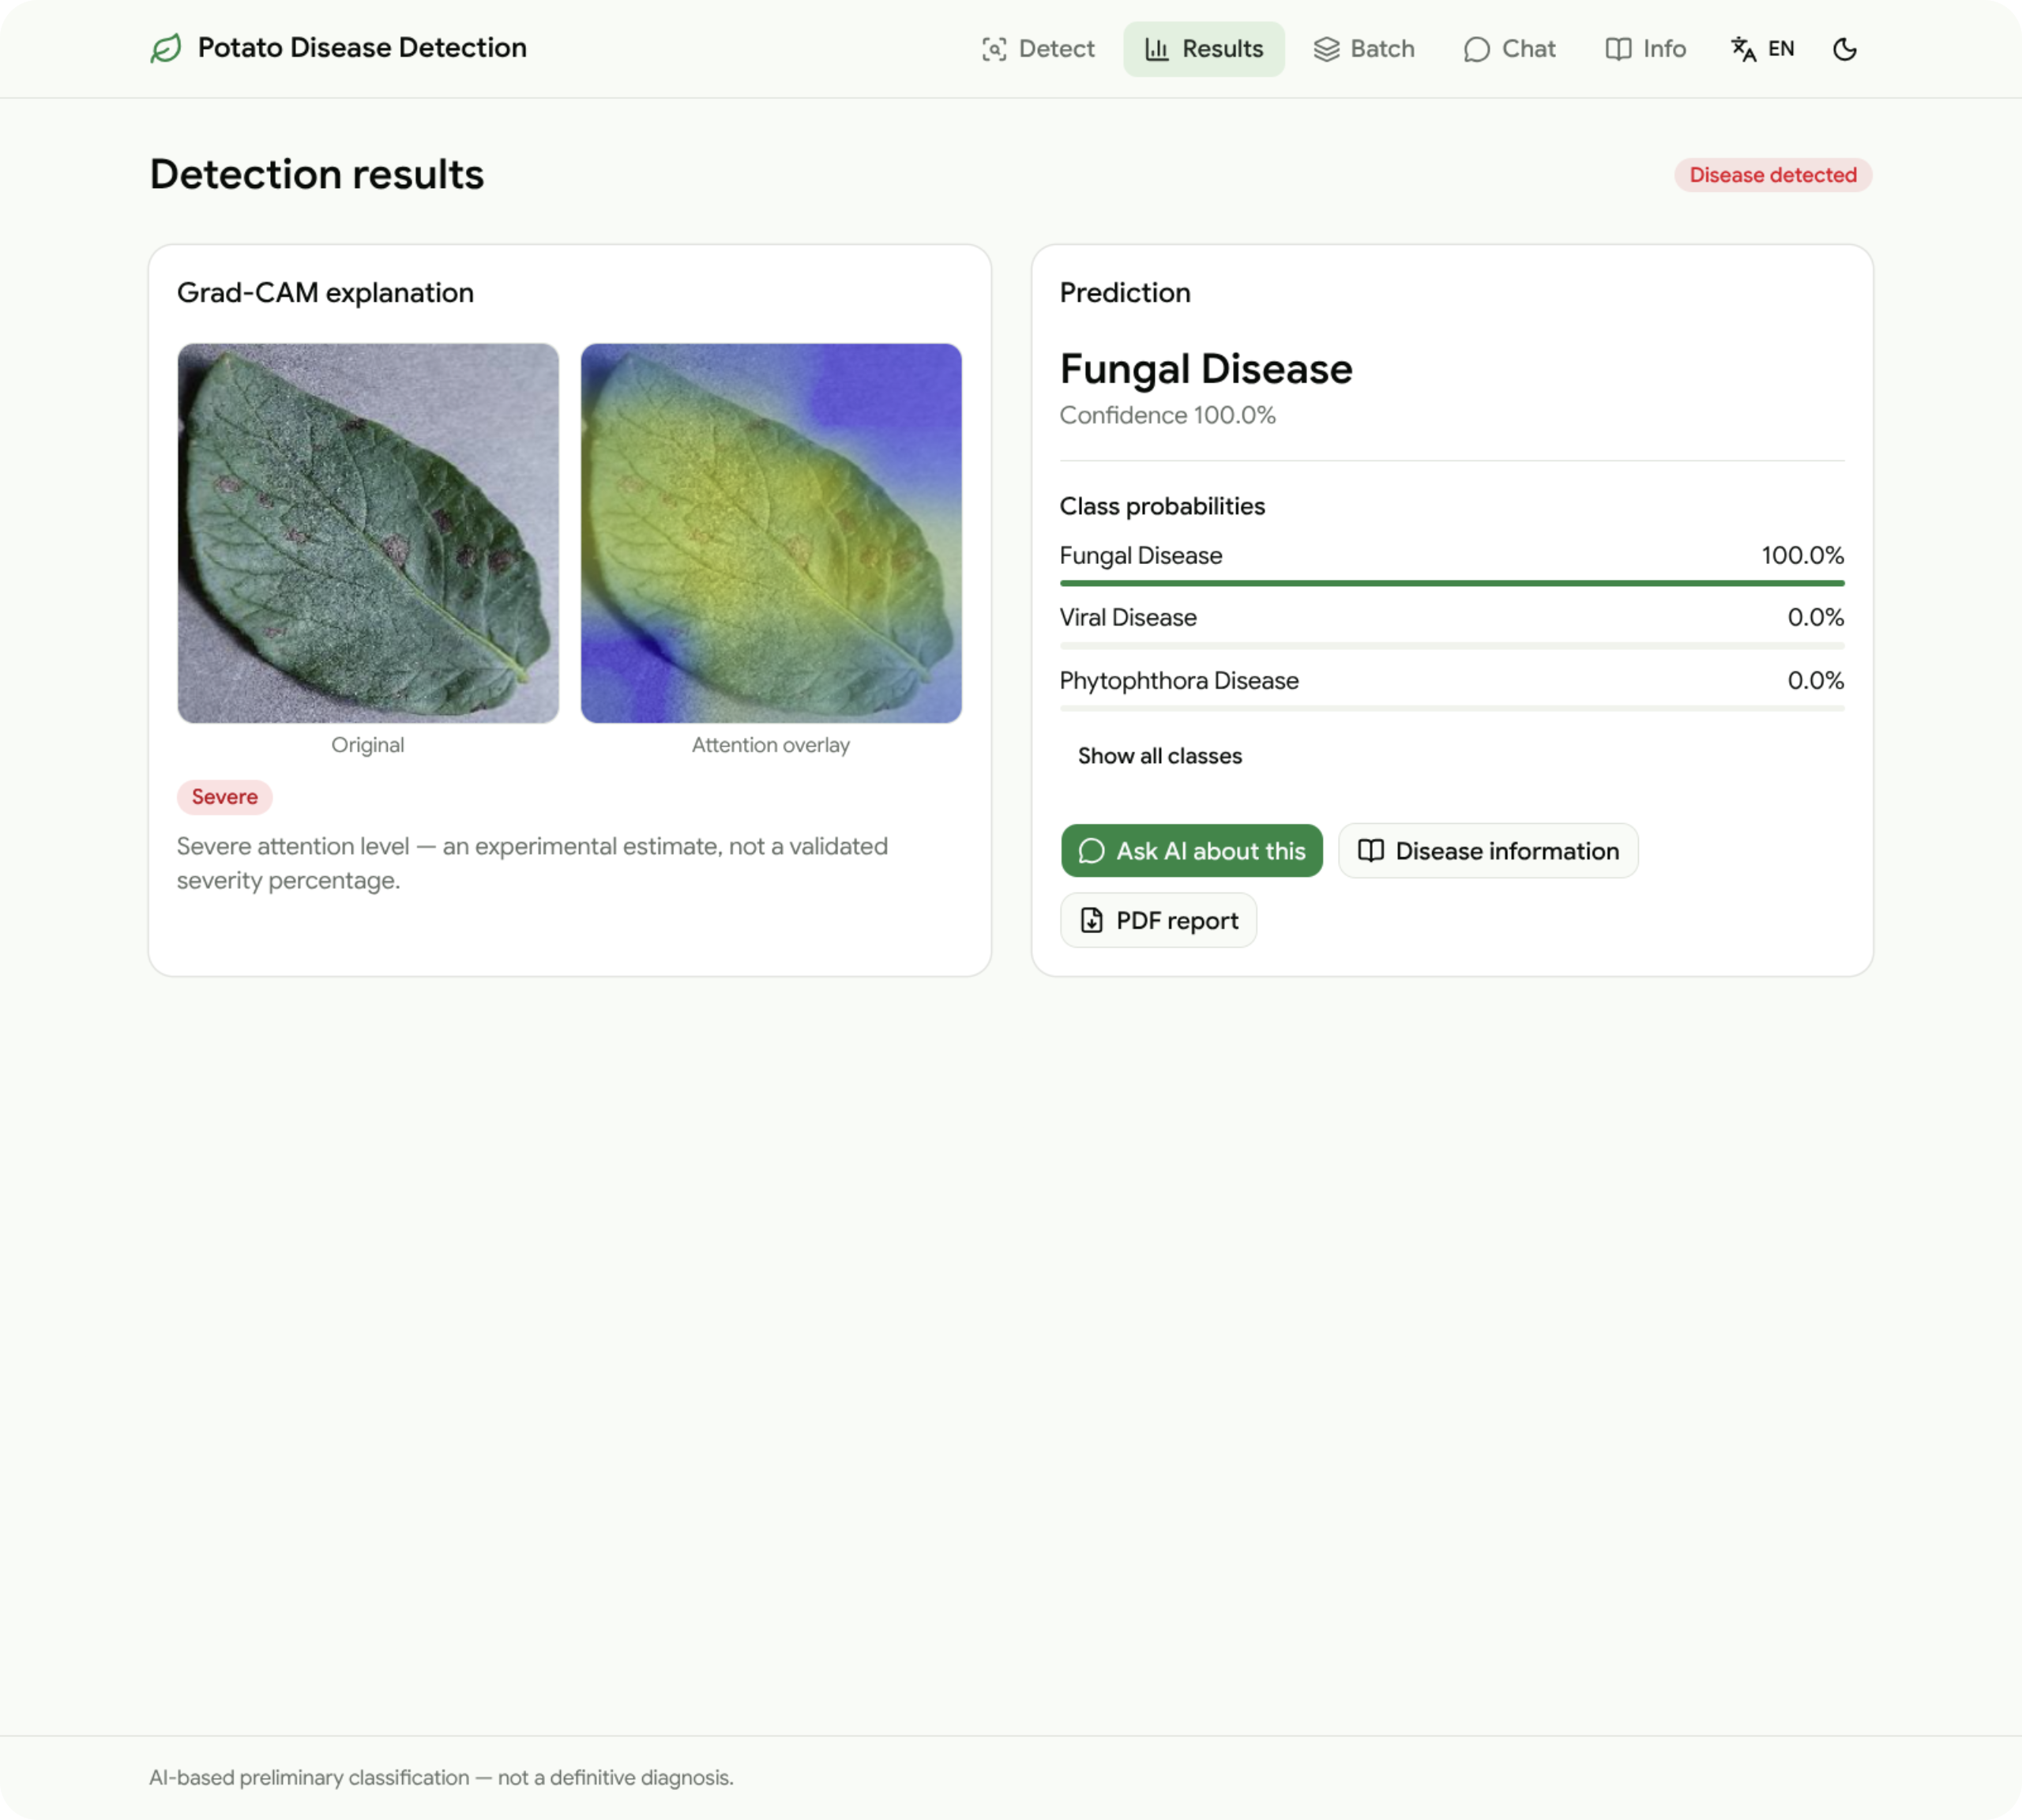
\includegraphics[width=0.92\textwidth]{image/Detection results.png}
\caption{\textit{Results} page displaying predicted class, top-class probabilities, side-by-side Grad-CAM attention overlay, experimental attention level, and PDF report export.}
\label{fig:webapp_results}
\end{figure}

\begin{figure}[htbp]
\centering
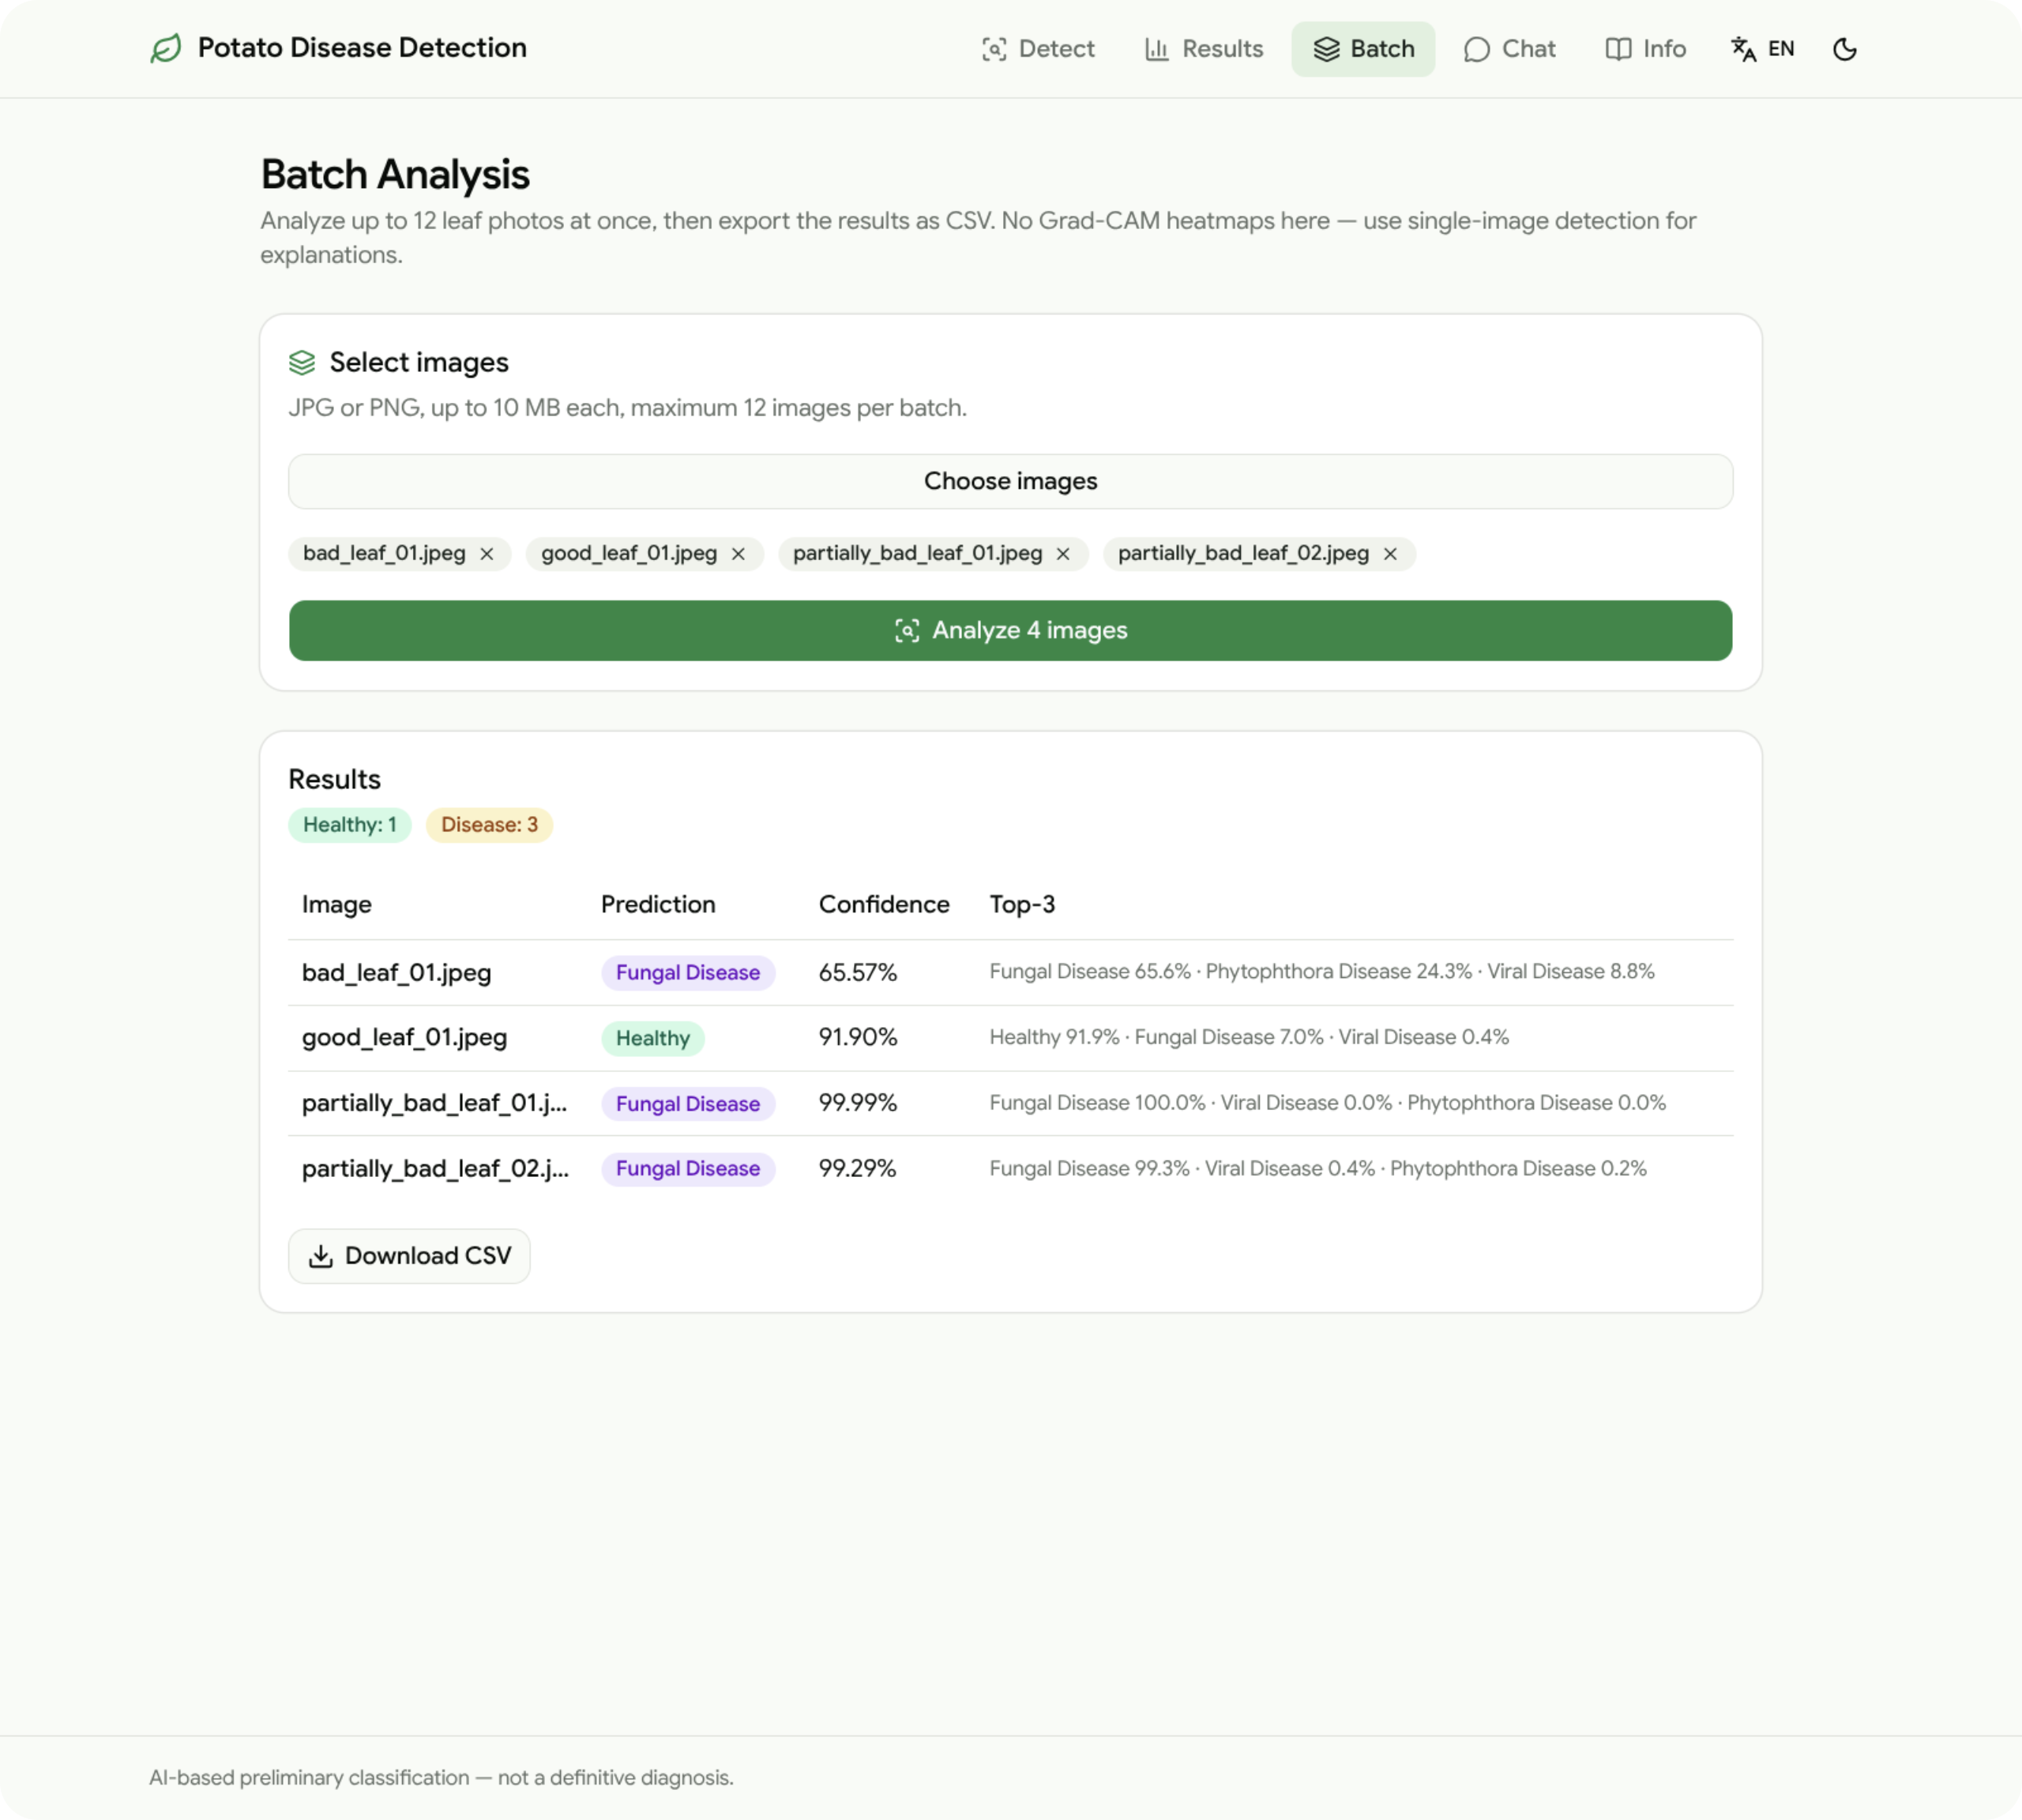
\includegraphics[width=0.92\textwidth]{image/Batch analysis.png}
\caption{\textit{Batch Analysis} page processing multiple leaf images simultaneously (up to 12 per batch) with Top-3 probability summaries and CSV export.}
\label{fig:webapp_batch}
\end{figure}

\begin{figure}[htbp]
\centering
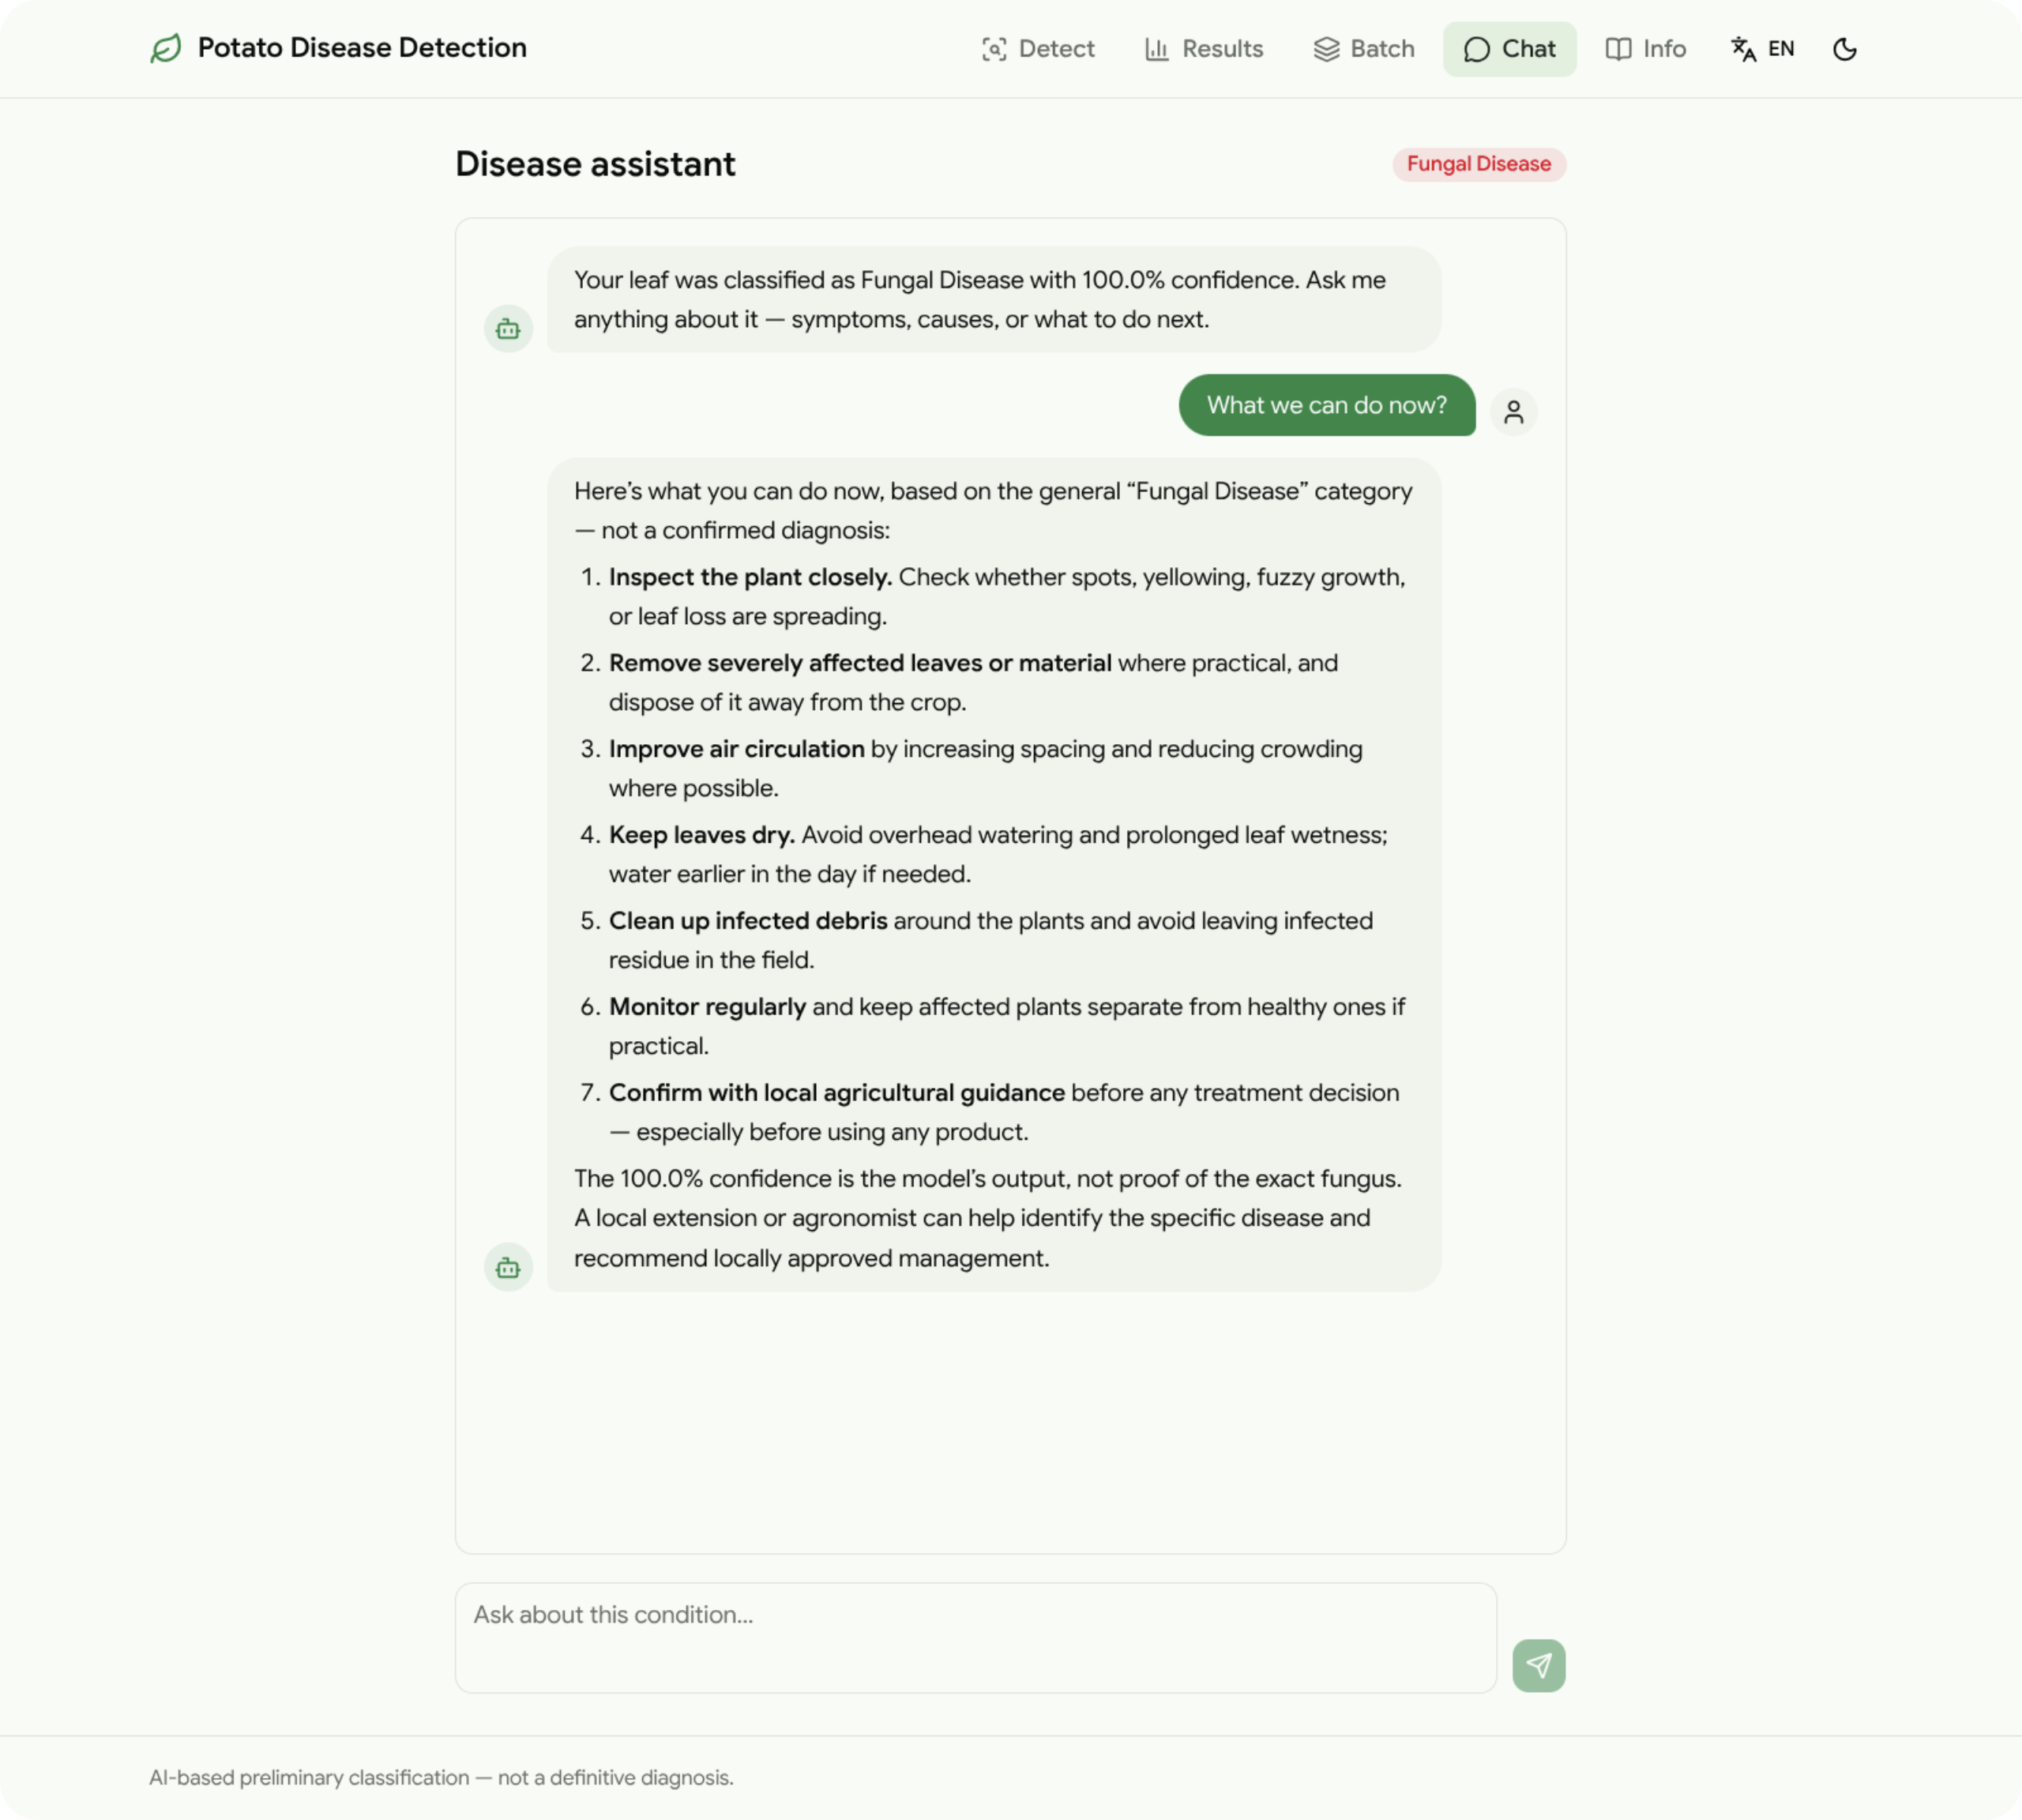
\includegraphics[width=0.92\textwidth]{image/Disease assistant - LLM.png}
\caption{Interactive bilingual (Bengali and English, Light and Dark modes) \textit{Disease Assistant} chat interface grounded in the classifier's prediction.}
\label{fig:ai_assistant}
\end{figure}

\begin{figure}[htbp]
\centering
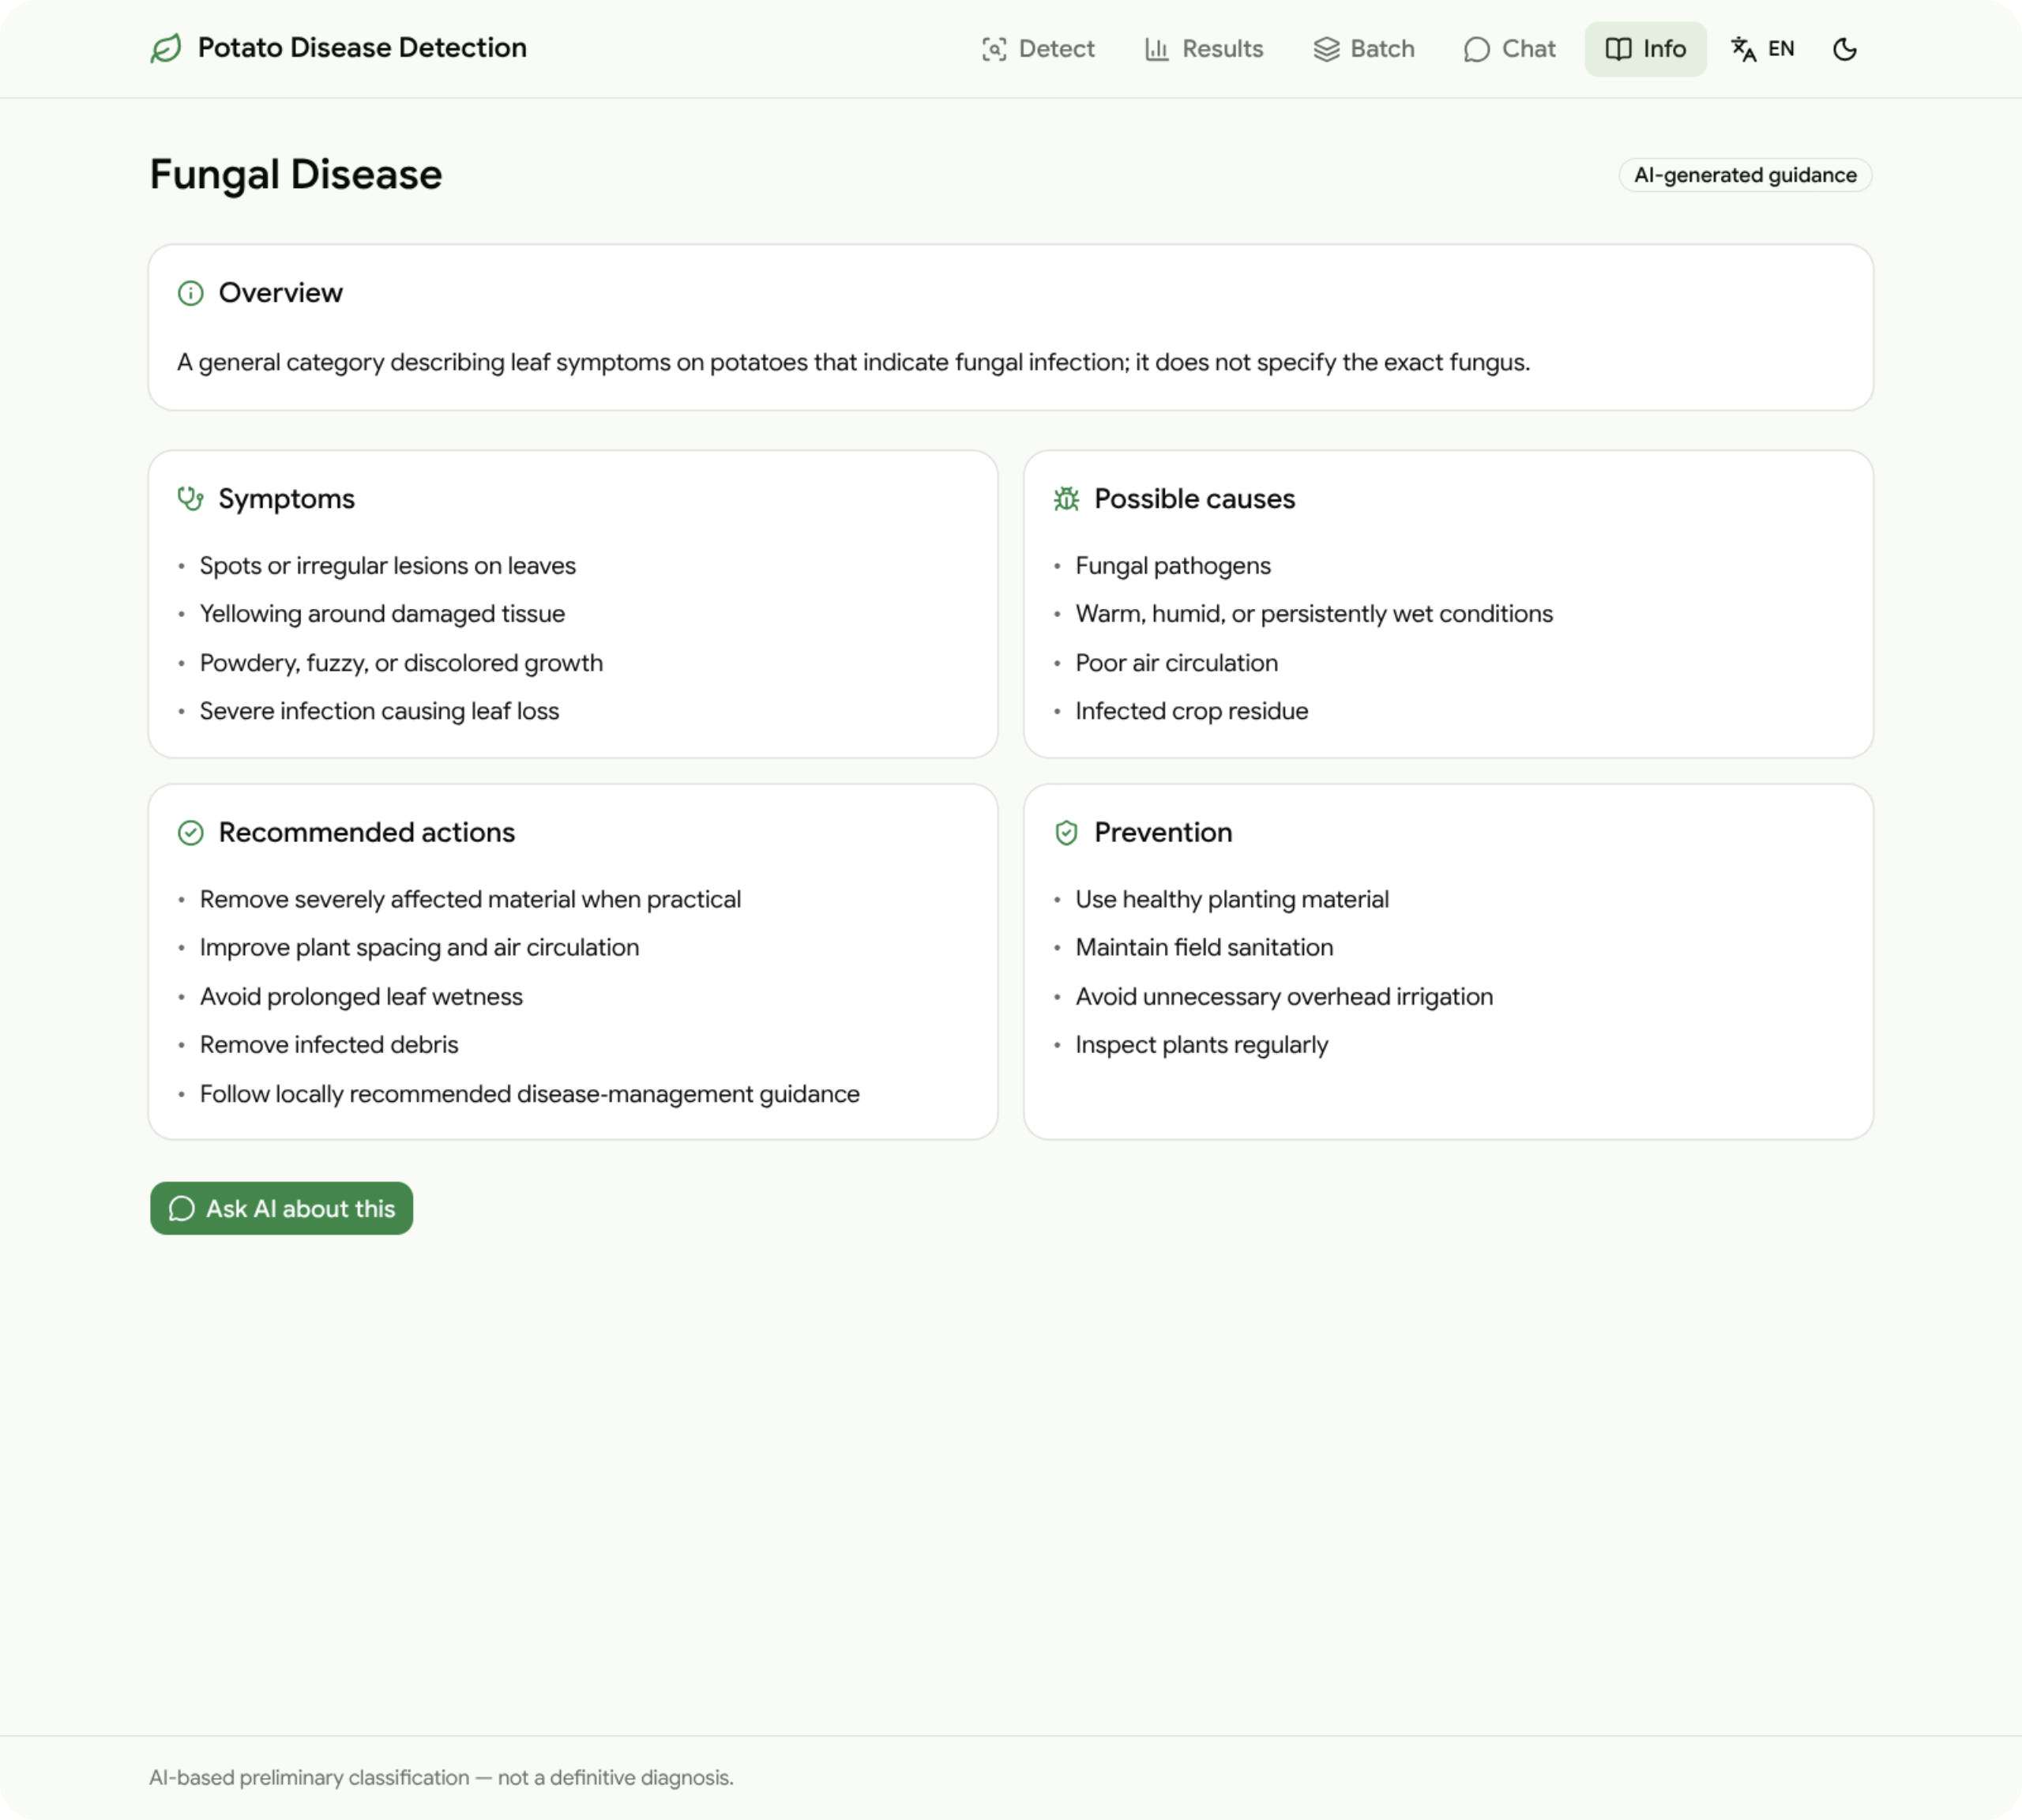
\includegraphics[width=0.92\textwidth]{image/Disease overview.png}
\caption{Structured \textit{Info} page presenting AI-generated Overview, Symptoms, Possible causes, Recommended actions, and Prevention cards.}
\label{fig:webapp_info}
\end{figure}

\subsection{Comparison with State of the Art Model}
Table~\ref{tab:final_summary} sums up the results and weight size of all three models on the identical 231 unseen test images. Figure~\ref{fig:acc_loss_comp} plots test accuracy and test loss.

\begin{table}[htbp]
\caption{Final Performance Summary on Test Set ($N = 231$)}
\label{tab:final_summary}
\begin{center}
\begin{tabularx}{\textwidth}{| X | c | c | c | c |}
\hline
\textbf{Model} & \textbf{Test Accuracy (\%)} & \textbf{Macro-F1} & \textbf{Test Loss} & \textbf{Model Size} \\
\hline
\textbf{Proposed MobileNetV2} & \textbf{93.51\%} & \textbf{0.9272} & \textbf{0.4466} & \textbf{8.64 MB} \\
\hline
MultiNet-V3 Ensemble & 90.91\% & 0.8975 & 0.6853 & 118.55 MB \\
\hline
InceptionV3 ($299 \times 299$) & 84.42\% & 0.8296 & 0.7353 & 85.18 MB \\
\hline
\end{tabularx}
\end{center}
\end{table}

\begin{figure}[htbp]
\centering
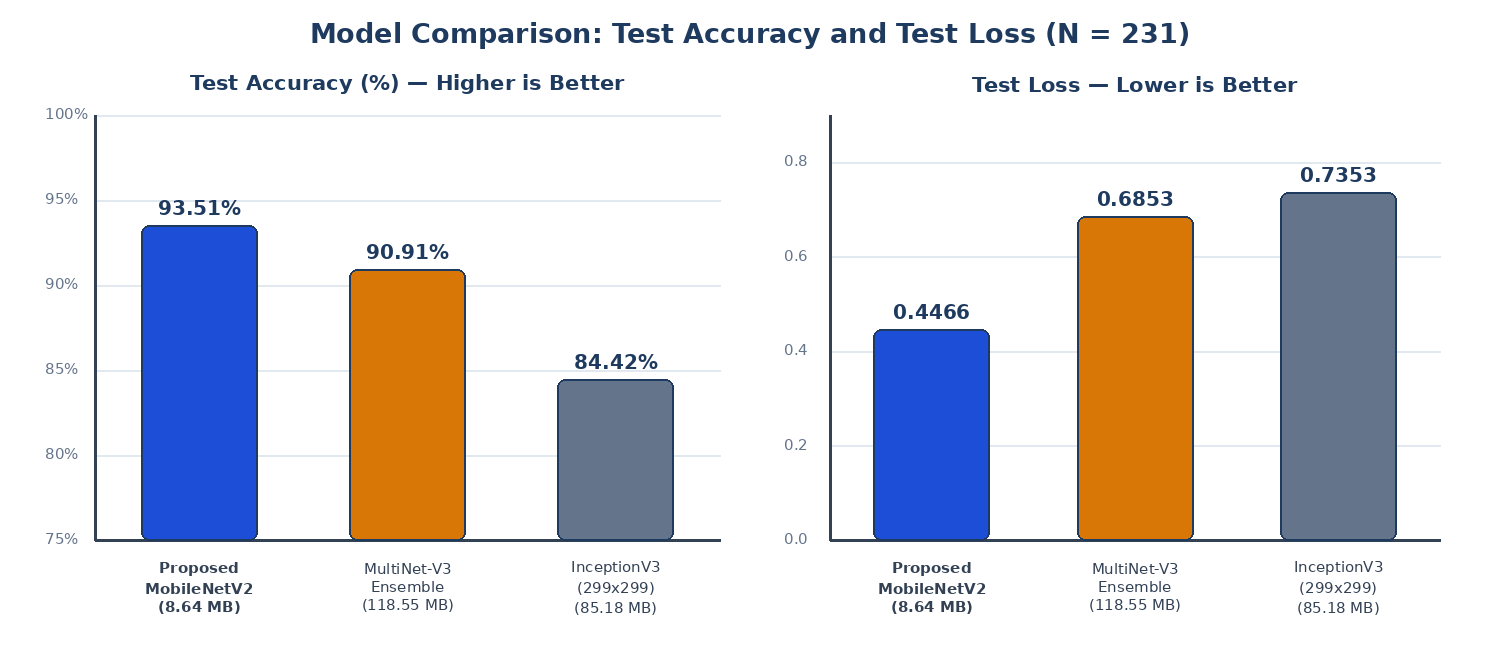
\includegraphics[width=0.92\textwidth]{image/comp_acc_loss.png}
\caption{Comparison of Test Accuracy and Test Loss across all three models. Proposed MobileNetV2 has the highest accuracy and lowest loss.}
\label{fig:acc_loss_comp}
\end{figure}

Figure~\ref{fig:radar} shows the per-class F1 comparison across all five biological classes: Proposed MobileNetV2 wins or ties on every single class (Bacterial 0.99, Viral 0.96, Fungal 0.91, Phytophthora 0.89, Healthy 0.88). The efficiency trade-off plot (Figure~\ref{fig:tradeoff}) shows that Proposed MobileNetV2 is both the smallest model (8.64~MB---$13.7\times$ smaller than MultiNet-V3 and $9.9\times$ smaller than InceptionV3) and the most accurate (93.51\%).

\begin{figure}[htbp]
\centering
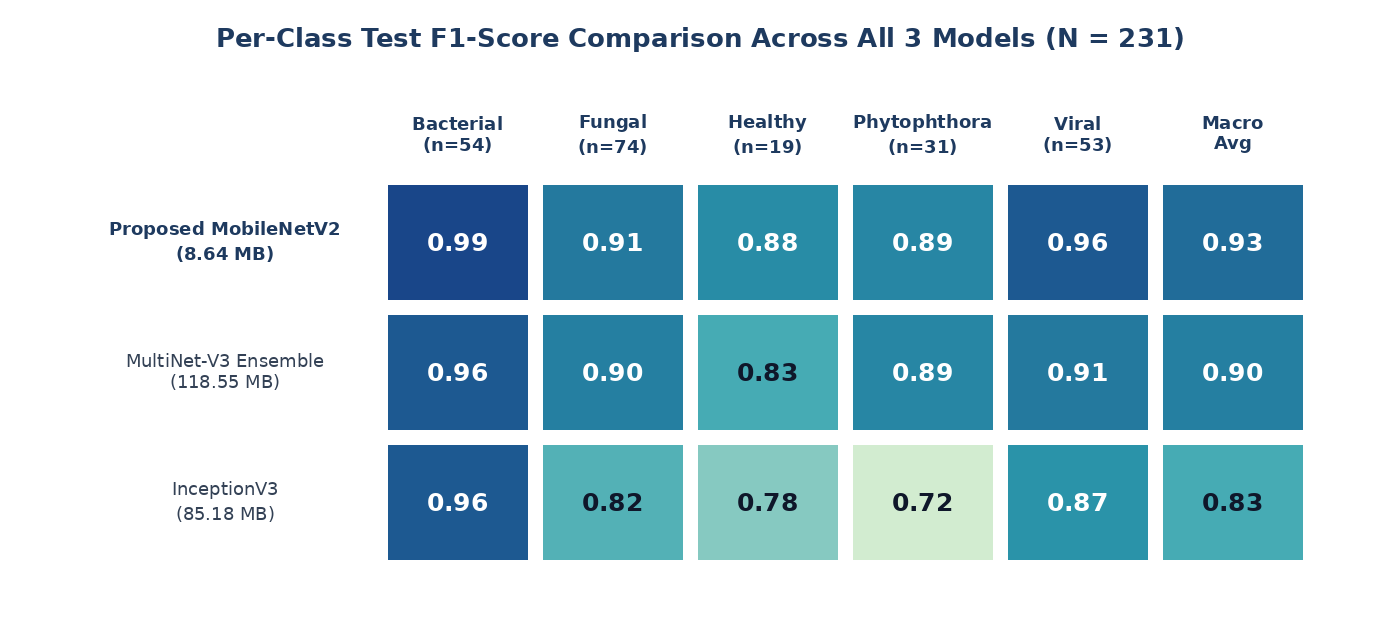
\includegraphics[width=0.92\textwidth]{image/comp_per_class_f1.png}
\caption{Per-class test F1-score heatmap across Proposed MobileNetV2, MultiNet-V3 Ensemble and InceptionV3.}
\label{fig:radar}
\end{figure}

\begin{figure}[htbp]
\centering
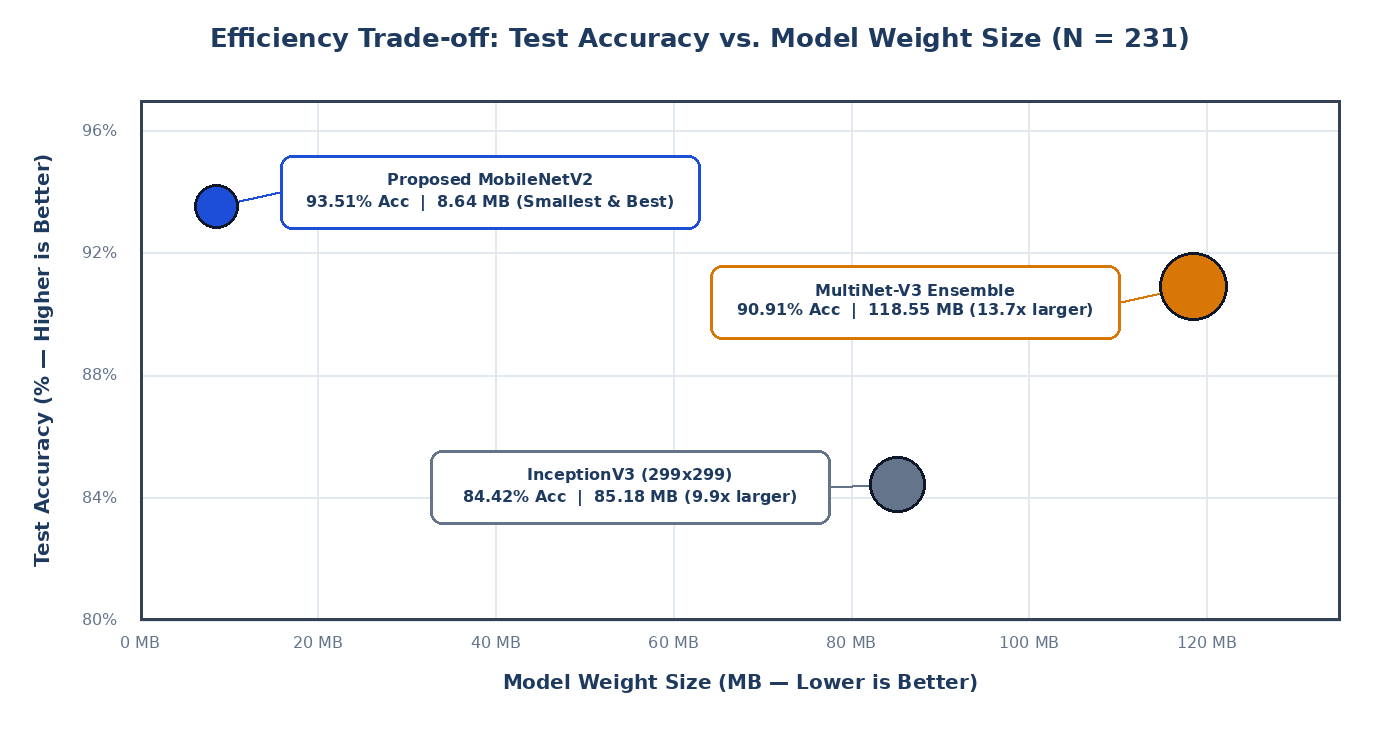
\includegraphics[width=0.88\textwidth]{image/comp_size_acc.png}
\caption{Efficiency Trade-off: Test Accuracy vs.\ Model Weight Size (MB).}
\label{fig:tradeoff}
\end{figure}

Table~\ref{tab:sota_comp} places our system next to well-known plant disease studies. Mohanty et al.\ \cite{mohanty2016using}, Sladojevic et al.\ \cite{sladojevic2016deep}, Ferentinos \cite{ferentinos2018deep} and Too et al.\ \cite{too2019comparative} reported very high accuracy on lab datasets with plain backgrounds, such as PlantVillage, using heavy models (up to $\sim 138$ million parameters) without XAI heatmaps or farmer LLM advice. Mohanty et al.\ \cite{mohanty2016using} and Shabrina et al.\ \cite{shabrina2024novel} showed that accuracy drops sharply on cluttered outdoor field photos. On our curated 5-class outdoor dataset, our compact 8.64~MB MobileNetV2 reaches 93.51\% accuracy while combining verified Grad-CAM explanations, safe bilingual Gemini guidance and a live web application.

\begin{table}[htbp]
\caption{Comparison of the Proposed Pipeline with State-of-the-Art Studies}
\label{tab:sota_comp}
\begin{center}
\scriptsize
\begin{tabularx}{\textwidth}{| p{2.3cm} | p{2.4cm} | p{2.3cm} | p{2.0cm} | p{1.6cm} | c | c |}
\hline
\textbf{Study} & \textbf{Dataset / Setting} & \textbf{Model(s)} & \textbf{Reported Outcome} & \textbf{Model Scale} & \textbf{XAI} & \textbf{LLM} \\
\hline
Mohanty et al.\ (2016) \cite{mohanty2016using} & PlantVillage (Lab, plain bg) & AlexNet, GoogLeNet & $>99\%$ (drops on field) & Heavy CNNs & No & No \\
\hline
Sladojevic et al.\ (2016) \cite{sladojevic2016deep} & 13 plant diseases & Deep CNN (CaffeNet) & Strong lab classification & Heavy CNN & No & No \\
\hline
Ferentinos (2018) \cite{ferentinos2018deep} & PlantVillage (58 classes) & VGG16, AlexNet, GoogLeNet & 99.53\% (VGG16) & $\sim 138$M params & No & No \\
\hline
Too et al.\ (2019) \cite{too2019comparative} & PlantVillage (fine-tuning) & DenseNet-121, ResNet, VGG & DenseNet-121 top performer & Moderate--Heavy & No & No \\
\hline
Shabrina et al.\ (2024) \cite{shabrina2024novel} & Uncontrolled Potato Field & Field benchmark dataset & Establishes field benchmark & Standard CNNs & No & No \\
\hline
\textbf{This Study (Proposed)} & Uncontrolled Potato (2,321, 5 cls) & MobileNetV2, MultiNet-V3, InceptionV3 & \textbf{93.51\%} (0.9272 F1) & \textbf{2.26M (8.64~MB)} MobileNetV2 & \textbf{Yes} & \textbf{Yes} \\
\hline
\end{tabularx}
\end{center}
\end{table}
